\documentclass{cacthesis}
\usepackage[ruled,vlined]{algorithm2e}
\usepackage{tabularx}
\usepackage{caption}
\usepackage{listings}
\usepackage{xcolor}
\usepackage{pifont}% http://ctan.org/pkg/pifont
\usepackage{amssymb}% http://ctan.org/pkg/amssymb
\newcommand{\cmark}{\ding{51}}%
\newcommand{\xmark}{\ding{55}}%

\newcounter{protocol}
\newenvironment{protocol}[1]
  {\par\addvspace{\topsep}
   \noindent
   \tabularx{\linewidth}{@{} X @{}}
    \hline
    \refstepcounter{protocol}\textbf{Protocol \theprotocol} #1 \\
    \hline}
  { \\
    \hline
   \endtabularx
   \par\addvspace{\topsep}}

\newcommand{\sbline}{\\[.5\normalbaselineskip]}% small blank line

\begin{document}

	\frontmatter
	
	%%%%%%%%%%%%%
	%% Title page
	%%%%%%%%%%%%%
	\title{Fair Exchange Protocol over Bitcoin}
	\author{Leandro Rometsch}
	\date{March 16, 2021}
	\subject{Bachelor Thesis}
	
	\publishers{
		\small
		\begin{tabular}{r l}
			Supervisors: &  Prof. Sebastian Faust, Ph.D. & & Benjamin Schlosser
		\end{tabular}
	}
	\maketitle
	
	\section*{Abstract}
    	The fair exchange of digital goods between two parties usually requires a trustee that is commonly realized today through smart contracts operating on cryptocurrencies like Bitcoin and Ethereum. Utilizing their decentralized nature in this context comes with the advantage of eliminating the single point of failure that a centralized, supposedly trusted third party implies. Because of its rich feature set, Ethereum is prominently used to realize smart contracts that imitate such a trusted third party. Bitcoin's rudimentary smart contracts do not receive as much consideration for the specific use case of fair exchange protocols as Ethereum does. These rudimentary smart contracts cannot hold any state, which requires a protocol design with minimal on-chain and additional off-chain logic. Hence, current fair exchange protocols on Bitcoin usually require heavyweight cryptographic primitives like zero-knowledge proofs or come with a lack of a high fairness guarantee. However, it is notable that Bitcoin enjoys a lot of media attention and offers the highest number of users, therefore increasing a fair exchange protocols' acceptance and economic potential. This thesis studies the relevant aspects of using Bitcoin as a trusted anchor for fair exchange without requiring heavyweight cryptographic primitives while maintaining fairness. In this context, we introduce an efficient protocol for the fair exchange of digital goods using Bitcoins rudimentary payment transactions. Our solution comes with two advantages: (1) The digital good's size only briefly affects the average transaction fees, and (2) cheap cryptographic operations like symmetric encryption schemes are sufficient for its execution. We implement different scenarios to evaluate our protocol's real-world costs. We show that the protocol is especially desirable in its optimistic case because its costs are entirely independent of the digital good's size. On the one hand, we conclude that the protocol is not directly realizable on current Bitcoin versions today, although it might be possible in the future. On the other hand, we discover that our protocol is desirable to run on related blockchain systems like Bitcoin Cash.
	
	\tableofcontents
	    
	\mainmatter
	
	\chapter{Introduction}
        %Sum up the basics of a data exchange protocol. Talk about the possibilities of smart contracts, how they can realize data exchange protocols, and why Bitcoin based smart contracts might be a good alternative to Ethereum based ones. 
        We describe an exchange scenario, where a buyer $B$ is willing to spend money in exchange for a product offered by seller $S$. $B$ expects the product to be in a particular condition beforehand. In a traditional setting, where both parties and the product are physically available at one place, $B$ can check for himself before paying if the product he planned to buy is the way $B$ expected it to be. If the expectation is not met, $B$ will not pay for the product - if it is, the exchange can be completed with minimal risk because both parties can be held liable. Neither $B$ nor $S$ got any disadvantage. \\
        This procedure is not trivially transferable to a digital setting - especially if digital goods are being exchanged. We assume $B$ wants to buy a digital product $d$, e.g., a song or a movie, and still got a certain expectation beforehand - this expectation is met if the predicate $\sigma\left( d\right) =1$. The dilemma is the following: Either $S$ needs to reveal its digital commodity $d'$ first to let $B$ check if $\sigma\left( d'\right) =1$, or B needs to pay beforehand without being able to inspect $d'$. Without trust among the two parties, this is undoubtedly vulnerable to fraud, and trust is not an ideal requirement in a digital setting where liability is limited. There are no security cameras, witnesses, nor is police on hand. One way to solve this dilemma is to introduce a middleman, some kind of trusted third party (TTP) to the exchange - similar to Certification Authorities that issue digital certificates. The TTP can independently verify if $B$'s expectation $\sigma$ is fulfilled and secure a fair exchange. Unfortunately, a dedicated middleman comes with significant drawbacks: A service like this is usually expensive, both parties need to agree on a specific one, and the availability is questionable. \\\\
        Cryptocurrencies offer huge potential here, with their \textit{smart contracts} imitating the middleman. A smart contract enables the transfer of money conditionally. The buyer and the merchant do not need to trust a single entity anymore. The only construct to trust is the decentralized \textit{blockchain} of the used cryptocurrency that evaluates a smart contract's conditions. The main difficulty here is that memory is financially limited on the \textit{blockchain} via fees. The naive approach of letting a smart contract evaluate $\sigma\left( d'\right)$, s.t. $\sigma$ is the condition to execute the monetary transfer, is only feasible if $d'$ consists of a few bytes but practically fails for larger files due to high fees - especially because digital items are usually relatively inexpensive. Another point to consider is that everything on the \textit{blockchain} is public. Therefore the naive approach is surely not advantageous for $S$. Using \textit{smart contracts} that support the cheap and private exchange of larger files (as an alternative to expensive TTP) requires a different protocol design - there are good solutions out there, but more on this in the next section.   \\\\  
        For a fair exchange protocol building on a particular cryptocurrency, an important aspect is the number of users the currency got. Choosing a cryptocurrency with a big user base increases the acceptance of the protocol. The most prominent technologies here are Bitcoin\footnote{https://bitcoin.org/en/} and Ethereum\footnote{https://ethereum.org/en/}. They both offer two completely distinct approaches when it comes to the construction of \textit{smart contracts}. Ethereum, on the one hand, offers a powerful virtual machine that enables the formulation of complex conditions and, therefore, powerful protocols via its statically-typed and object-oriented programming language. On the other hand, Bitcoin only supports basic payment transactions based on a simple stack-based scripting language. Usually, fair exchange protocols utilizing Bitcoin are less efficient or lack a high fairness guarantee. \\\\
        This thesis aims to analyze whether it is possible to construct an efficient and cheap fair exchange protocol on top of Bitcoin rather than most other protocols achieving these properties utilizing Ethereum. A solution is particularly interesting because it would make cheap fair exchange accessible for a broader market while potentially reducing the complexity on the \textit{blockchain} itself.
        % Move this into the contribution section: Therefore, we will look into efficient Ethereum based protocols and investigate the possibility of transferring one to Bitcoin, making it accessible for a broader market.
        
        \section{Related Work}
        \label{sec:relatedWork}
        All efficient approaches to our exchange scenario have in common that they use the \textit{blockchain} as a trusted anchor and only utilize it when necessary to minimize costs. The credo is that the computation done by the participating parties locally is usually much cheaper (but not necessarily negligible) and, therefore, preferred against expensive computation done by the smart contract. \\\\
        The fair exchange protocols utilizing Bitcoin usually choose computationally demanding zero-knowledge proofs \cite{zkcp}\cite{DELGADOSEGURA2020832}, mainly because of the limitations Bitcoins \textit{smart contracts} have. Other approaches, primarily Ethereum based ones, try to avoid these computational burdens while simultaneously keeping the protocol participants' fees low. FairSwap \cite{10.1145/3243734.3243857}, for example, enables buyer $B$ to prove misbehavior of a merchant afterward instead of checking $\sigma$ beforehand. Optimistic protocols like this one are advantageous because they usually only need to perform costly \textit{blockchain} interaction if fraud is suspected, making the optimistic case very cheap. The cheap optimistic case is highly desirable, especially if there is no incentive for one of the parties to cheat. One way to remove any incentive, also concerning Denial of Service (DoS) attacks, is to introduce unavoidable penalties when misbehaving. \\\\
        The crucial part of every fair exchange protocol is how to design $\sigma$, or informally speaking, the \textit{data correctness proof} s.t. $B$ can verify for itself that the product advertised by $S$ is the expected one. Different approaches do this either before or after the data exchange. Delagado et al. use a cut-and-choose technique in the first phase of their Bitcoin-based protocol \cite{DELGADOSEGURA2020832}, which splits the file into many single but still meaningful chunks. E.g., if $B$ expects to buy a specific movie from $S$, the movie is split up into chunks of its frames. A small subset of these frames is manageable for $B$ to verify beforehand, which gives (depending on the size of the subset) $B$ the confidence to proceed in the exchange. FairSwap does this the other way around by assuming a public fingerprint is available for every digital item being exchanged. After the actual file exchange, $B$ then computes the fingerprint on his own and compares it to the public one. If they do not match, $B$ can prove this to the protocol through the (TTP imitating) smart contract and get a refund. Section \ref{sec:FairSwap} goes into more details on FairSwap.

        \section{Environments}
        \label{sec:smartContractOptions}
        In this section, we want to take a quick look at the properties of Bitcoin, Bitcoin Cash\footnote{https://www.bitcoincash.org/}, and Ethereum in terms of using them as a smart contract foundation. \\
        In contrast to Bitcoin and Bitcoin Cash, Ethereum offers the \textit{Turing-complete} Ethereum Virtual Machine (EVM). It is similar to typical virtual machines like Java's JVM and can solve any (solvable considered) problem only limited by the given resources. Each EVM operation is given a specific price to calculate the fees the owner of a submitted smart contract must pay to the network. This fee is termed \textit{gas}, and the \textit{gas limit} restricts an Ethereum smart contract's complexity. The most popular language utilized to write \textit{smart contracts} using the EVM is Solidity\footnote{https://docs.soliditylang.org/en/v0.8.0/}. Solidity is a high-level language that is influenced by C++, Python, and JavaScript. By submitting an Ethereum smart contract, a special deployment transaction is published that contains the contract's bytecode but no receiver. All public functions of a smart contract are natively accessible via the Application Binary Interface (ABI). Besides interaction via the ABI, \textit{smart contracts} can communicate with other \textit{smart contracts}. This enables decentralized applications with an unlimited number of participants. Because of the flexible and powerful EVM, Ethereum, e.g., creates the foundation of the current surge of decentralized finance (DeFi) applications like Compound\footnote{http://compoundcoin.org/} and Uniswap\footnote{https://uniswap.org/}. \\\\ 
        These advanced uses of \textit{smart contracts} are not possible with Bitcoin. There is no \textit{Turing-completeness}, and notably, the \textit{smart contracts} cannot hold any state because all data is only temporarily stored onto a stack during execution (Section \ref{sec:BTC} explains this in detail). Bitcoin chose this design intentionally to allow the efficient and independent verification of transactions. Although this design limits the on-chain possibilities, there are certainly ways to extend these possibilities by combining transactions with off-chain logic. \\\\ 
        Bitcoin Cash benefits from Bitcoins attributes by using the same underlying structure but enables additional functionality by (re-)introducing more complex operations. Storing data on Bitcoins Cash \textit{blockchain} is much cheaper and, in contrast to Bitcoin, encoding and decoding of data is possible. There are also high-level languages available that enable state simulation, e.g., Solidity inspired CashScript\footnote{https://cashscript.org/}, to build \textit{smart contracts} on top of Bitcoin Cash. \\\\
        All three cryptocurrencies come with their up and downsides. Ethereum trades efficient validation for extensive functionality. Bitcoin focuses on a rudimentary stateless version of \textit{smart contracts} to increase independence and validation efficiency. Bitcoin Cash builds on this and aims to find a compromise here.
            
            
    \chapter{Preliminaries}
        \section{Bitcoin}
        \label{sec:BTC}
        In 2008 Satoshi Nakamoto proposed the first practical decentralized peer-to-peer currency system (commonly known as "cryptocurrency"), named Bitcoin (BTC) \cite{nakamoto2009bitcoin}. The premise of Bitcoin is a shared data structure maintained by a decentralized network of nodes. This data structure is made out of cryptographically chained blocks, the so-called \textit{blockchain} (cf. §\ref{sub:Blockchain}), that miners continuously work on extending. One new block added to the \textit{blockchain} allows for a certain amount of new payment transactions and simultaneously increases the integrity of the blocks before. Other cryptocurrencies might extend their \textit{blockchain} differently. However, in Bitcoin's case, this \textit{proof-of-work} approach is used, such that the \textit{blockchain}'s integrity is guaranteed, as long as the honest nodes control more than half of the networks computational power\footnote{Computational power is necessary to generate new \textit{blockchain} blocks - it is also known as \textit{hash rate}. If one party alone controls more than half of the \textit{hash rate} new blocks can easily be manipulated}. For the computational burden the miners take, they are compensated with newly generated Bitcoins and transaction fees. The result is a self-sustaining system that is decentralized and trustable. From a high level, Bitcoin can be considered as an emulated trusted bank without a single entity controlling it. The trust in Bitcoin is high because there were practically no successful attacks yet. This fact is essential for the acceptability of a decentralized currency system because no central institution could be held liable. Simultaneously this increases the acceptance of Bitcoins \textit{blockchain} to act as an TTP through \textit{smart contracts}. The users' trust rests in the \textit{proof-of-work} consensus protocol that secures the validity of transactions and prevents double-spending. \\\\
        It is notable that Bitcoins \textit{blockchain} stores transactions of Bitcoins (and some metadata to secure the \textit{blockchain}) and only implicitly the user's balances. The name Bitcoin might be misleading here because there are no actual coins, only a traceable path of transactions that originate from a miner's reward. The amount of Bitcoin one person owns can be calculated by looking at every transaction this person received but did not spend jet. If a person wants to perform a Bitcoin transaction, it needs access to one key pair containing one public key and one private key. The public key is essentially the person's address, which enables him/her to receive Bitcoins. The private key is needed to send Bitcoins to other users' public keys. Because everybody can create arbitrary key-pairs without providing any personal information, Bitcoin provides some anonymity for its users. \\
        The introduction of Bitcoin, especially the \textit{blockchain} concept, kickstarted many other cryptocurrencies and \textit{blockchain}-based applications. Still, Bitcoin is the most widely accepted cryptocurrency and remains the largest by market capitalization\footnote{Source: \url{https://coinmarketcap.com/} (14.12.2020)} - followed by Ethereum and XRP.

        \subsection{BTC Transactions}
        \label{sub:BTCTx}
        
        Technically there are no Bitcoins, only transactions of a particular Bitcoin value that are either spent or unspent. Each new transaction needs at least one input transaction. The sum of the value of all input transactions determines the maximum value of the new transaction. The remaining amount of Bitcoin value inside a transaction (Bitcoin that is not targeted to an address) is used as a transaction fee. The higher the fee, the faster the transaction is being processed by the network. Once a transaction is published in a new block on the \textit{blockchain}, its input transaction(s) are considered spent. A new transaction itself is unspent until it is again used for some other valid transaction as input. Only unspent transactions can be used as an input transaction. If one of the input transactions is already spent, the new transaction is recognized as invalid and rejected by the network. \\
        The other two essential parts of every Bitcoin transaction are the out script and the witness. The out script is an cryptographic puzzle that contains the condition(s) that need to be fulfilled by somebody that wants to spend the transaction. The witness is the values that are given as input to the out script. Consequently, the out script is the lock of a transaction, and the witness is the key. Note that the witness inside a transaction is not related to its own out script - it is needed to unlock the out script of the input transaction(s). Therefore, if the user knows the correct values to fulfill the out script of an unspent transaction, it practically owns the particular Bitcoins. Take Figure \ref{fig:tx1} as an example. The out script is written in Bitcoin's scripting language and is usually utilized to perform standard payments to a single Bitcoin address (\textit{P2PKH}, explained in \ref{sub:BTCScript}). More complex out scripts are possible that enable payments under a wide variety of conditions, e.g., timelocks or the signatures of multiple users.
        \begin{figure}
          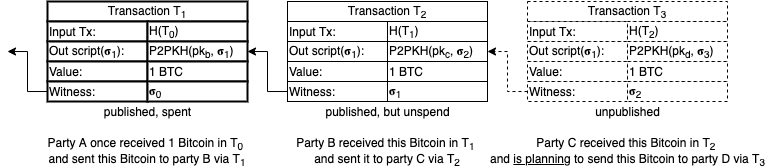
\includegraphics[width=\linewidth]{images/basic_transaction_figure.png}
          \caption{Example of a Bitcoin transaction trace.}
          \label{fig:tx1}
        \end{figure}
        \\\\ For an efficient transaction validity check, each node stores, in addition to the \textit{blockchain} (or checkpoints of it), two transaction pools locally: The \textit{pending transaction pool} and the \textit{unspent transaction pool}. Pending transactions are valid transactions requested for execution but are not included in a \textit{blockchain} block yet. If a node receives a new valid transaction from a user, the node puts it into its \textit{pending transaction pool} and forwards it to all connected peers. Once a new block is added to the \textit{blockchain}, a node deletes all transactions the new block contains from its \textit{pending transaction pool} and updates its \textit{unspent transaction pool}. Suppose a node wants to evaluate the validity of the input transactions of a new transaction. In that case, it checks if all input transactions are available in the \textit{unspent transaction pool} - if this is not the case, the new transaction is rejected. This procedure ensures that a node does not need to search through the whole \textit{blockchain} each time a new transaction is submitted. \\

        \subsection{BTC Script}
        \label{sub:BTCScript}
        
        Bitcoin Script is the scripting language every transaction out script is formulated in. It formalizes the conditions that have to be met (given the witness as input) to spend a specific transaction. The two significant characteristics of Bitcoin Script are its \textit{Turing-incompleteness} and the stack-based evaluation. The out script's possibilities are very limited because of the \textit{Truing-incompleteness} (especially compared to the EVM). Loops or jumps are not possible. This property's advantage is that endless loops (or, in general, deadlocks) are being avoided. Therefore, attack vectors for DoS attacks are limited. Malicious parties cannot create complicated transactions and slow down the Bitcoin network. The stack-based approach makes a Bitcoin Script very efficient to be evaluated - especially storage wise. When running a script, its elements are pushed on and popped out of the stack in a Last In First Out (LIFO) manner. The script is written in postfix notation and processed from left to right; therefore, e.g., $3\ OP\_ADD \ 4$ will appear as $3\ 4\ OP\_ADD$. Any Bitcoin Script is considered valid if no opcode triggers any failure, and after the evaluation, the top item on the stack is true. \\
        Bitcoin Scripts opcodes can be divided into several categories: From constants, flow control, or stack operations over arithmetic to cryptographic ones. In Table \ref{tbl:opcodes} we will list a few, to our contribution and general understanding relevant, opcodes. The full list is available at the Bitcoin Wiki\footnote{https://en.bitcoin.it/wiki/Script}. Over time, many opcodes were disabled because of security and efficiency concerns. However, it is also possible that new opcodes are added via \textit{soft forks}. A \textit{soft fork} is Bitcoin's way of improving its protocol. Anybody can propose these Bitcoin Improvement Proposals (BIP) and, if widely accepted by the network, the protocol is updated accordingly. \\\\
        Let us showcase a very common Bitcoin Script. Most Bitcoin transactions are direct transactions from one party to another (scenarios like, e.g., in Figure \ref{fig:tx1}). The out script used in these cases is the Pay to Pubkey Hash (\textit{P2PKH}). Instead of including the receiver's public-key, only the hash of the receiver's public-key is deposited. The procedure supports anonymity and hinders brute-force attacks. The receiver unlocks the out script by providing his signature of the transaction and his public-key. Thereby it can be proven that the receiver owns the private-key related to the public key and indeed wants to spend this exact transaction by providing the proper signature. The \textit{P2PKH} script, is available in Listing \ref{lst:p2pkh}. \textit{ScriptPubKey} is representing the cryptographic puzzle itself, while \textit{scriptSig} is describing the input parameters. Figure \ref{fig:p2pkh} showcases the stack during an exemplary successful execution step-by-step. The \textit{P2PKH} script is easily expendable to the \textit{MultiSig} script, which consequently requires multiple parties to successfully unlock the out script and spend the transaction. \\
        
        \definecolor{backcolour}{rgb}{0.95,0.95,0.92}
        \begin{lstlisting}[language=JavaScript, basicstyle=\footnotesize, caption=Bitcoin \textit{P2PKH} script, captionpos=b, backgroundcolor=\color{backcolour}, label=lst:p2pkh]
        scriptPubKey: OP_DUP OP_HASH160 *pubKeyHash* OP_EQUALVERIFY OP_CHECKSIG
        scriptSig: <sig> <pubKey>
        \end{lstlisting} \\
        
        Besides the \textit{P2PKH} and the \textit{MultiSig} script, numerous other powerful (but less popular) scripts exist. Especially interesting for exchange protocols are Hash-Lock scripts. These enable to challenge a potential receiver to provide some data that results in the hardcoded hash (in exchange for the Bitcoin value). Be aware that transactions like this are not necessarily secure on their own. A network node could theoretically drop the transaction and unlock it independently with the legitimate receiver's data. By combining the Hash-Lock script with the \textit{P2PKH} script, personalizing it to the receiver, the described vulnerability is fixed. \\
        The final script we want to mention here is the Hashed-Timelock script. It works accordingly to the Hash-Lock script but adds a timelock. The transaction's sender can unlock the script on his own, in the case the timelock expired and the receiver did not unlock the script by providing data matching to the hash. Usually, in Bitcoin Script, timelocks are denoted by a specific block number. If this block number is reached, the timelock is triggered. Bitcoins block numbers are easy to predict because they increment by one, and usually, it takes around 10 minutes until a new block is found. \\\\
    
        \begin{figure}
          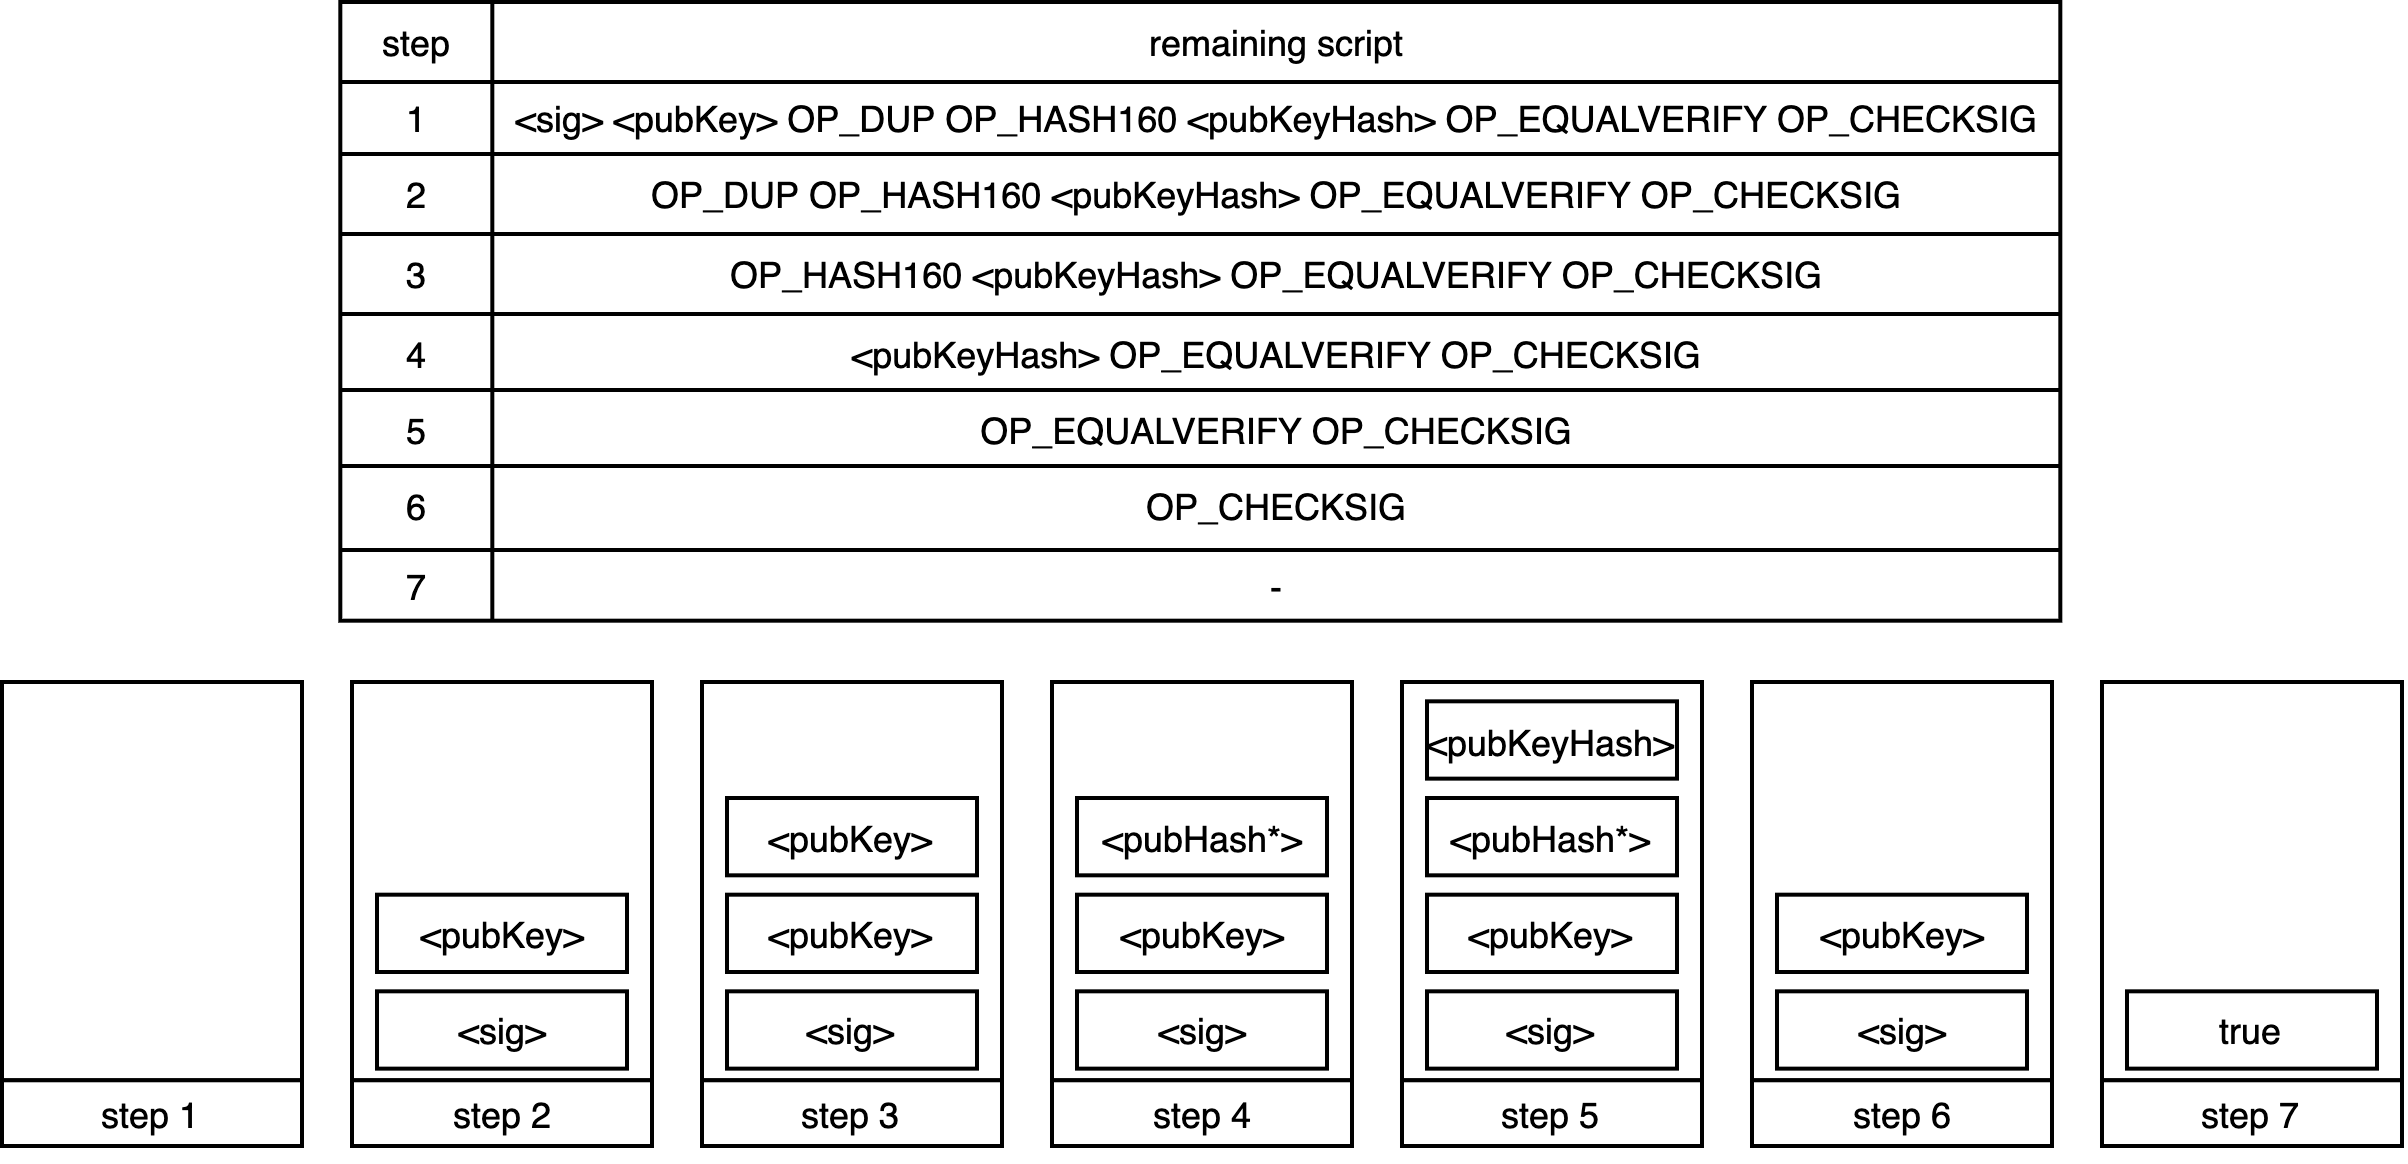
\includegraphics[width=\linewidth]{images/p2pkh_execution_figure.png}
          \caption{Stack visualization of a Bitcoin \textit{P2PKH} script execution.}
          \label{fig:p2pkh}
        \end{figure}

        \begin{center}
            \begin{tabular}{ l | l | c | c }
             Operation  & Description & BTC & BCH \\ 
             \hline
             OP\_DUP & Duplicates an element & \cmark & \cmark \\
             OP\_HASH160 & Performs SHA-256 and then RIPEMD-160 & \cmark & \cmark  \\
             OP\_EQUAL & Compares two values and returns 1 if equal & \cmark & \cmark \\
             OP\_VERIFY & Marks execution as invalid if top value is not true & \cmark & \cmark \\
             OP\_EQUALVERIFY & Performs (1) OP\_EQUAL and (2) OP\_Verify & \cmark & \cmark \\
             OP\_CHECKSIG  & Compares the transaction hash to given signature & \cmark & \cmark \\
             OP\_CAT  & Concatenates two elements &  \xmark & \cmark \\
             OP\_XOR  & Calculates bitwise exclusive or & \xmark & \cmark \\
            \end{tabular}
            \captionof{table}{Some Bitcoin Script opcodes}
            \label{tbl:opcodes}
        \end{center}
        
        \subsection{Bitcoin Cash}
        \label{sec:BitcoinCash}
        Bitcoin Cash is a \textit{hard fork} of Bitcoin. In contrast to the usual BIPs that are implemented via \textit{soft fork}, there is the chance that the Bitcoin network is split over a major controversial BIP, which would make old blocks of the \textit{blockchain} incompatible. If no agreement is achieved and enough nodes of the network support the BIP, the part of the network agreeing could choose to extend the \textit{blockchain} with the new version on their own, while the other part of the network extends with the old protocol - resulting in a \textit{hard fork}. \\
        In 2017 this happened with Bitcoin Cash emerging from Bitcoin. Bitcoin Cash increased the block size limit from 1 MB to 8 MB. Additionally, Bitcoin Cash supporters did not support various BIPs to come, most prominently BIP141\footnote{https://github.com/bitcoin/bips/blob/master/bip-0141.mediawiki} (commonly known as \textit{SegWit}). The overall goal was to increase the possible transactions per time to use the cryptocurrency as a proper replacement for fiat money and not for investment purposes. In 2018 the block size limit increased again to 32 MB, enabling the currency to theoretically perform up-to 130 transactions per second (Bitcoin manages around 5 transactions per second). Bitcoin Cash also reintroduced various Bitcoin Script opcodes that were previously disabled by BIPs in Bitcoin. For this thesis, relevant ones are noted in Table \ref{tbl:opcodes}. The extended opportunities of Bitcoin Cash over Bitcoin in the context of \textit{smart contracts} are laid out in Section \ref{sec:smartContractOptions}. \\\\
        Bitcoin Cash's fundamental advantage is the much higher throughput of transactions, which implicitly brings down the cost per transaction (= transaction fee). The general criticism is focused on the supposedly naive solution of increasing the block sizes instead of finding efficient off-chain solutions or improvements to the protocol itself. It is also noteworthy that Bitcoin's network contains many more nodes than Bitcoins Cash network and that Bitcoin enjoys a higher acceptance, therefore serves a broader marked.
        
        \section{FairSwap}
        \label{sec:FairSwap}
        We already mentioned that \textit{smart contracts} on the \textit{blockchain} could imitate the role of a TTP. Dziembowski et al. use this characteristic in their FairSwap protocol \cite{10.1145/3243734.3243857} and offer an exemplary Ethereum based implementation\footnote{https://github.com/lEthDev/FairSwap}. Like other fair exchange protocols, the underlying goal is to guarantee the seller S to receive a payment from buyer $B$ if $S$ delivers the product $x$, s.t. the buyer's expectation formalized as the circuit (= predicate) $\sigma$ is met. This circuit must consist of simple operations to maintain efficiency. Although the TTP is imitated with the smart contract, interaction is still expensive. Especially, the evaluation of large circuits is costly. To avoid this, Dziembowski et al. observe that it is much cheaper to prove $S$'s misbehavior after the exchange and not before via verifying $\sigma(x)$ fully. While this makes the protocol very efficient, it limits FairSwap to two participating parties and makes it non-interactive. \\\\
        In the first step of the exchange, the smart contract is initialized, and $S$ is encoding $x$ (which is divided into $n$ parts) with a secret key $k$. The encoded $x$ is sent off-chain to $B$, who can then buy $k$ from $S$. The smart contract forms a trusted anchor by storing $\sigma$ and other essential values like the cryptographic fingerprint of $x$. These values are public, and after their verification, $B$ can be confident of receiving $x$ or at least a refund. Once $B$ paid and $k$ is revealed by $S$, $B$ will run the extraction procedure by decrypting encoded $x$ and verifying it with $\sigma$. Note that $\sigma$ got $n$ inputs, each one being a part of $x$. If the circuit fails, \textit{concise proof of misbehavior} is generated. This proof contains a piece of the circuit $\sigma$ that does not return an expected intermediate gate value. $B$ can submit this proof to the smart contract, verifying if the intermediate value is indeed incorrect. Therefore, if this is the case, $S$'s misbehavior is publicly proven, and $B$ automatically receives a refund. \\\\
        Notably, this exchange protocol does not use any heavy cryptographic tools like \textit{zero-knowledge proofs}. The main cryptographic primitives utilized are cryptographic hash functions, commitment schemes, and symmetric encryption. The implementation of FairSwap employs Merkle trees as an efficient to evaluate circuit. These primitives are relatively easy to compute. For a circuit with $m$ gates, the smart contract got a complexity of $O(log(m))$ and the computation costs for both parties are $O(m)$. The smart contract's \textit{gas costs} and each party's computational burden are dependent on the number of chunks $x$ is divided in (= $n$). The larger each chunk (therefore $n$ being smaller), the higher the \textit{gas costs} but, the smaller the local computational burden. While the local computational burden is independent of the exchange's success or failure, the \textit{gas costs} rise if \textit{concise proof of misbehavior} is submitted because this implies additional computation inside the smart contract. Therefore, for the pessimistic case, the \textit{gas costs} rise exponentially with an increased chunk size. \\\\
        Through the powerful EVM, it is possible to realize this protocol with only one smart contract to verify all potential \textit{concise proof of misbehavior}.
        FairSwap is further optimizable by utilizing off-chain state channels and integrating penalties into the contract, s.t. possible DoS attacks of S are monetarily limited, which could temporarily lock B's coins. These penalties also relativize the high pessimistic costs for big chunks because the optimistic case's probability rises, bringing the average costs down.
                
        \section{Cryptographic Primitives}
        \label{sec:CryptoPrimitives}
	        \subsection{Hash Functions}
	        \label{sub:HashFunctions}
	        Cryptographic hash functions take a string of arbitrary length as input and map it onto a fixed-sized one. We assume the hash function $H:$ $ (0, 1)^*$ $\rightarrow$ $(0, 1)^p$  is a one-way function and collision resistance (for large enough p), s.t. the outcome can informally be considered the input's unique cryptographic fingerprint. 

            \subsection{Symmetric Encryption Scheme}
            \label{sub:SymmetricEncryptionScheme}
	        The encryption scheme utilized in this thesis is a xor cipher. The secret key k is generated through a pseudo-random number generator (denoted $k$ $\leftarrow$ $(0, 1)^n$). The ciphertext is calculated by concatenating k with an index value i (denoted $k\|i$), hashing it and calculating  $c = m \ \oplus \ H(k\|i)$. We calculate the reversal $m = c \ \oplus \ H(k\|i)$ to reveal the plaintext again. \\
            Although this simple scheme is known to be vulnerable to frequency analysis and known-plaintext attacks, it suits our contribution because the encrypted data is not necessarily containing written language, and k is newly generated for every protocol run.

            \subsection{Merkle Tree}
            \label{sub:MerkleTree}
	        The Merkle tree is a data structure that enables efficient data validation. It is a fundamental building block of many popular \textit{blockchains} like Bitcoin or Ethereum. \\
            It is also called a hash tree because it utilizes cryptographic hash functions to create a tree of hash values with data chunks as leaves. The parent nodes combine their two children by concatenating and hashing again. We give an example of a Merkle tree in Figure \ref{fig:merkleTreePrelims}. The root of the Merkle tree implicitly acts as a cryptographic fingerprint of all leaves combined. We denote the root of a Merkle tree $M$ as $root(M)$ and the $sibling$ of node $v$ is the value the node is being hashed with to create the $parent$ (e.g. in Figure \ref{fig:merkleTreePrelims}: H$_1$ is the $sibling$ of H$_2$ with both having H$_5$ as $parent$). Further, we say that $leaf_i$($M$) results in the $i$-th leaf of Merkle tree $M$ (e.g. in Figure \ref{fig:merkleTreePrelims}: $leaf_1$($M$)$=$ H$_1$). Note, that the leaves are hashed before the tree is created. There are utilizations of Merkle trees that directly concatenate the leaves. \\
            We will use the algorithms \textsf{Mtree}, \textsf{Mproof}, and \textsf{Mvrfy} also utilized by Dziembowski et al. in \cite{10.1145/3243734.3243857}. \textsf{Mtree} (Algorithm \ref{algo:Mtree}) generates the Merkle tree of a n-tuple $(x_1, ..., x_n)$. For simplicity we require $n$ to be a power of two. \textsf{Mproof} (Algorithm \ref{algo:Mproof}) takes value $i$ and generates the proof that $x_i$ is the $i$-th leaf of \textsf{Mtree(x)}. \textsf{Mvrfy} (Algorithm \ref{algo:Mvrfy}) receives a Merkle root, a Merkle proof and a leaf and verifies if the leaf is indeed part of the corresponding Merkle tree based on the given proof. 
            
            \begin{figure}
            \begin{center}
              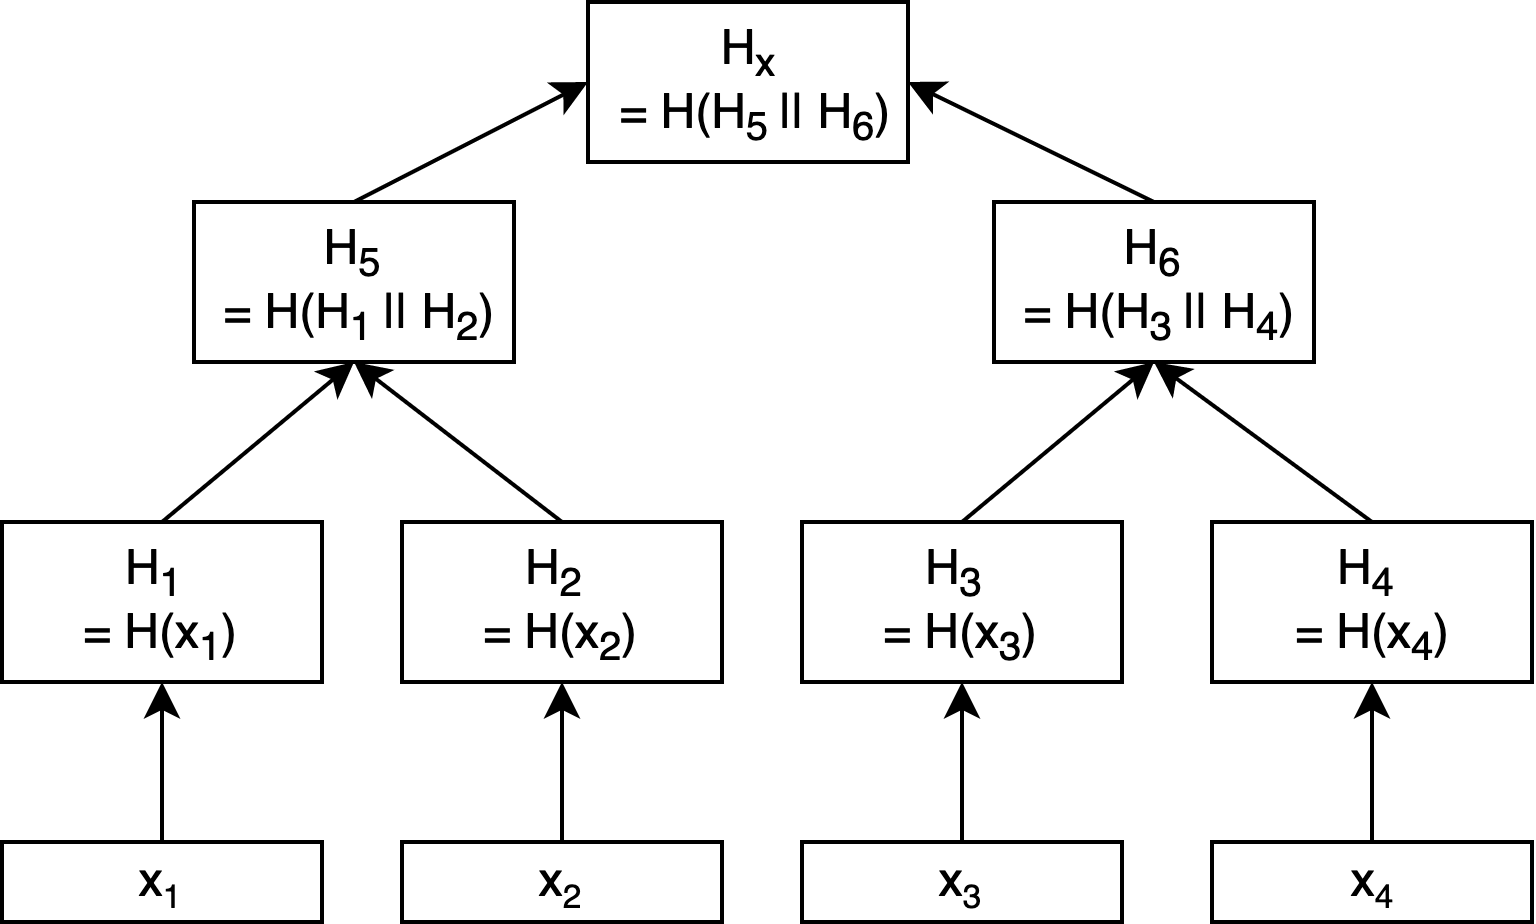
\includegraphics[width=0.6\textwidth]{images/merkle_tree_figure.png}
              \caption{Merkle tree with root $H_x$ for $x = (x_1, x_2, x_3, x_4)$.}
              \label{fig:merkleTreePrelims}
            \end{center}
            \end{figure}
        
        \begin{center}
        \begin{minipage}[t]{4in}
            \begin{algorithm}[H]
                 \If{$n = 1$}{
                    $R = H(x_1)$\;
                 }
                 \Else {
                    $v_0^l = \textsf{Mtree}(x_1, ..., x_{n/2})$\;
                    $v_0^r = \textsf{Mtree}(x_{n/2 + 1}, ..., x_n)$\;
                    $R = H(root(v_0^l)\|root(v_0^r))$\;
                 }
                \Return MerkleTree $M$ with root $R$\;
                \caption{\mbox{Create Merkle tree: \textsf{Mtree}(Leaves \textit{$x_1, ...,x_n$})}}
                \label{algo:Mtree}
            \end{algorithm}
        \end{minipage}
        \end{center}   
        
        \begin{center}
        \begin{minipage}[t]{4in}    
        \begin{algorithm}[H]
                \textbf{set} $v = leaf_i$($M$) \;
                \ForEach{$j \in [log_2(n)]$}{
                  \textbf{set} $l_j = sibling$ of $v$\;
                  \textbf{set} $v = parent$ of $v$\;
                 }
                 
                \Return MerkleProof $(l_1, ..., l_d)$\;
                
                \caption{Create Merkle tree proof: \\ \textsf{Mproof}(MerkleTree $M$, Index $i$)}
                \label{algo:Mproof}
            \end{algorithm}
        \end{minipage}
        \end{center}
        
        \begin{center}
        \begin{minipage}[t]{4in}
            \begin{algorithm}[H]
                \ForEach{$l_j \in p$}{
                    \If{$i/2^j = 0$ $ mod $ $2$}{
                    $x = H(l_j\|x)$\;
                    } \Else{
                    $x = H(x\|l_j)$\;
                    }}
                \If{$x = h$}{
                    \Return $1$\;
                 } \Else{
                    \Return $0$\;
                 }
                \caption{Verify Merkle tree proof: \\ \textsf{Mvrfy}(Leave $x$, MerkleProof $p = (l_1, ..., l_d)$, Root $h$)}
                \label{algo:Mvrfy}
            \end{algorithm}
        \end{minipage}
        \end{center}
        
        \subsection{Blockchain}
        \label{sub:Blockchain}
        
        The blockchain itself is a simple data structure consisting of cryptographically connected data chunks ("blocks"). Most prominently, it is utilized as the shared data structure of many current cryptocurrency systems like Bitcoin (cf. §\ref{sec:BTC}) to store all transactions in a decentralized ledger. Most notably, the data stored on the blockchain must be immutable to e.g., prevent double-spending or stealing of coins. It must be (negligibly) hard to replace, delete, or modify any block and, therefore, the included transactions. The chaining of blocks achieves immutability through cryptographic hash functions. We stress that the deeper a block is integrated into the (continuously extending) blockchain, the stronger is the immutability property of this particular block. E.g., in Bitcoin, it is recommended to wait for six confirmations (= six blocks) until a transaction is confidently regarded as integrated into the blockchain. We informally construct the following three functions to provide simplified communication with the blockchain for our protocol participants. Without the loss of generality, we assume a transaction is confirmed once its public and its conditions are valid. \\\\ 
        \textsf{PublishToLedger(tx)} takes a transaction \textsf{tx} (e.g., a Bitcoin transaction as defined in Section \ref{sec:BTC}) and publishes it to the ledger. It returns \textit{true} if \textsf{tx} was successfully added to the ledger and \textit{false} if \textsf{tx} got rejected (e.g., because the \textit{out script} of \textsf{tx} input transaction failed as described in Section \ref{sub:BTCTx}). For the sake of simplicity, this function does not take a witness for the input transaction of  \textsf{tx}. \\\\ 
        \textsf{Claim(tx, [args])} creates and publishes a \textit{P2PKH} transaction with \textsf{tx} as its input transaction and the caller being the receiver. \textsf{[args]} is the witness to unlock the out script of \textsf{tx}. Therefore, the function returns \textit{true} if the out script succeeded and the caller claimed the funds locked in \textsf{tx}. The function returns \textit{false} if the out script of \textsf{tx} failed. For the sake of simplicity, we ignore signatures as arguments in \textsf{[args]}.\\\\ 
        \textsf{IsOnLedger(tx)} verifies if a transaction \textsf{tx} is already integrated into the ledger. If \textsf{tx} is additionally not spend, the function will return \textit{true}. If \textsf{tx} is not on the ledger or is already used as input for another transaction (e.g., like $T_1$ in Figure \ref{fig:tx1}), the function will return \textit{false}.
        


        

    \chapter{Fairness in Exchange Protocols}
    \label{sec:Fairness}
        Bentov and Kumaresan state that a fair exchange protocol is a particular subcase of secure multiparty computation \cite{10.1007/978-3-662-44381-1_24}. Numerous multiparty computation protocols achieve a notion of security that is capturing a form of fairness. One common way of defining fairness, in this case, is \textit{if one party receives their expected output, then so do all} \cite{10.1007/978-3-540-79263-5_8}. Cleve showed in \cite{10.1145/12130.12168} that it is impossible to achieve this notion of fairness when there is no honest majority among the protocol participants. Let us carry this knowledge into the context of a two-party exchange protocol: At the point where there is one dishonest party involved, it is impossible to achieve the mentioned form of fairness. Consequently, it is crucial to specify acceptable alternative notions of fairness specially tailored for the two-party case.   \\\\
        The obstacle when using the idea of \textit{fairness} is that various interpretations among different points of view exist. Markowitch et al. stated that it is crucial for defining fairness in exchange protocols to focus on what fairness is and not on how to obtain it \cite{10.1007/3-540-36552-4_31}. It is obvious to claim that a \textit{fair} exchange protocol requires that no party gains a \textit{significant advantage} over the other party. Different explanations of what is meant with a \textit{significant advantage} result in different fairness notions. \\
        The primary definition commonly used among publications around fair exchange protocols (like \cite{10.1145/266420.266426} \cite{asyncOptiFairEx1998} \cite{remarksOnFairEx2000})  is the following: \textit{At the end of every exchange protocol run, either all involved parties obtain their expected information/asset, or none of them receives anything.} This definition might be satisfying in some scenarios, but \textit{advantage} is still described insufficiently and only focuses on the actual exchange result here. In other words, this definition could be interpreted as some superficial notion of fairness. \\\\
        We construct the following scenario: $B$, the buyer, and $S$, the seller, use a fair exchange protocol $\pi$ to trade some digital coins for a digital item. The high-level procedure of $\pi$ is as follows: $B$ locks up digital coins that $B$ is willing to spend for a particular digital item $d$ that satisfies the predicate $\sigma$ s.t. $\sigma\left( d\right) =1$. The digital coins can be redeemed by $S$ if $S$ can deliver a digital item $d'$ s.t. $\sigma\left( d'\right) =1$. If $S$ can do this, $B$ can be sure that $d' = d$ and both parties are satisfied. If $S$ is not responding with a matching $d'$, the previously locked-up coins will be available for $B$ again after a pre-defined timeframe $t$, and $S$ cannot claim them anymore. \\
        In the sense of the above-defined superficial notion of fairness, this protocol is fair because there are only two possible outcomes of $\pi$. Either the exchange succeeded, or non of the parties receives anything. 
        Although $\pi$ is certainly fair under this definition, $B$ got - depending on the point of view - a significant disadvantage. $B$ cannot use the coins for something else during the execution of $\pi$, and a malicious $S$ could use this knowledge, e.g., for a DoS attack. One could argue that this is not fair because one party got a \textit{significant advantage} over the other party. Therefore, giving definitions for different notions of fairness comes hand-in-hand with specifying the term \textit{advantage}. This is, unfortunately, missing in our mentioned superficial notion of fairness. 
        
        \section{Specifying Advantage}
        \label{sec:Advantage}
        While explaining \textit{advantage} in the context of fair exchange protocols, Markowitch et al. come up with three main aspects that make up different notions of fairness \cite{10.1007/3-540-36552-4_31}. (1) \textbf{General fairness}, directly relating to the items being exchanged during the protocol, s.t. \textit{at the end of every exchange protocol run, either all involved parties obtain their expected information/asset, or none of them receives anything}.  (2) \textbf{Timeliness}, relating to the ability of a single party to capture the progress of the protocol and the option to abort it at some point. (3) \textbf{Abuse-freeness}, in the sense that if there is an unsuccessful execution of the protocol, no party can show the validity of intermediate results to others. As a result, no single party alone can prove to an outside one that he has the power to terminate or complete the protocol successfully. This attribute is considered difficult to achieve (especially while preserving \textit{timeliness}), and only a few protocols attain it (e.g., \cite{Gao2008}). In general, a specific notion of fairness might consider one aspect stronger, weaker, or even irrelevant. \\
        Projecting these aspects on our protocol $\pi$ mentioned above: (1) is undoubtedly fulfilled because either the exchange succeeded or non of the parties receives anything. (2) is only partially fulfilled because $S$ might be able to abort by not responding, but $B$ must wait until the coins are unlocked. $B$ is also not able to capture the protocol's progress because $S$ might be preparing the transmission of $d'$ or already aborted. Either way, the protocol is time-wise limited by the pre-defined timeframe $t$. (3) is not fulfilled because there is no mechanism to stop $S$ from randomly aborting the protocol. If $S$ indeed owns $d'$ s.t. $\sigma\left( d'\right) =1$, $S$ can prove to an outside party that $S$ has the power to terminate or complete $\pi$ successfully, at least after $B$ locked the coins and until $B$ can unlock the coins again. $S$ can abuse $\pi$ for the only purpose of blocking $B$'s coins for a particular time - even if $S$ does not know $d$. 
        
        \section{Strong Fairness, Weak Fairness}
        \label{sec:StrongFairnessWeakFairness}
        Another common notion of fairness is \textit{Strong Fairness}, sometimes referred to as perfect fairness. Pagnia and Gärtner created an early formal definition for \textit{Strong Fairness} in exchange protocols \cite{Pagnia99onthe}. They are essentially stating that both parties expect the goods being exchanged to be in a particular condition or quantity, much like the predicate $\sigma$ of our example $\pi$. \textit{At the end of the protocol run, either both parties expectations are being fulfilled, or no information about the other party's respective good is gained.} This notion ensures that the exchange either succeeds or ultimately fails, with nothing in-between.
        It is worth mentioning that some publications expect from their notion of \textit{Strong Fairness} that, after a payment transaction, it must be possible for the buyer to successfully claim the original expected item in case of a dispute, without requiring the misbehaving seller to cooperate \cite{10.1007/3-540-36552-4_31}. Informally speaking: After payment, the exchange must succeed. For our imaginary protocol $\pi$, this is not the case and would require a different strategy. Usually, this is achieved by heavyweight trusted third parties (TTP). This TTP could take $d$ from $S$ as an initial step in $\pi'$ and check if the expectation $\sigma$ is fulfilled. $B$ only proceeds if the TTP approves. The protocol $\pi'$ could then run as defined in $\pi$ with the small addition that if $S$ is not providing $d$ until $t$ by itself, the TTP will send a copy of $d$ to $B$ and finish the exchange. However, there exist optimistic protocols using transparent TTP that are used to maintain this notion of \textit{Strong Fairness} \cite{10.1007/3-540-36552-4_31} \cite{6982058}. \\\\
        While in \textit{Strong Fairness} it is required that the exchange fully succeeded or failed, in \textit{Weak Fairness} this property is softened. 
        \textit{Weak Fairness} demands that it must be possible for an honest party to prove to an outside one that the opposite party received the expected item, while the complaining party did not. Although the proof is required, \textit{Weak Fairness} does not expect that the implicated dispute is resolvable. However, this information could potentially be used by some protocol to execute a refund mechanism. \\\\
        We want to stress that these two related flavors of fairness focus on the point of protocol termination. In contrast to this, the above-presented description of \textit{advantage} focuses on fairness during the protocol run itself.
        
        \section{Probabilistic Fairness}
        \label{sec:ProbabilisticFairness}
        Finally, there are fair exchange protocols that need to merge their notion of fairness with probability. These are usually protocols that depend on techniques that offer a probability of fairness (e.g., cut-and-choose in \cite{DELGADOSEGURA2020832}) based on the chosen security parameters. We recognize \textit{Probabilistic Fairness} as a relativization to already defined notions of fairness since most definitions can be easily shifted into a probabilistic context. Let us do this for our previously mentioned superficial notion of fairness: \textit{For an adequate security parameter k, at the end of the exchange protocol run, there must be a high enough probability that either all parties obtain their expected information or non of the parties obtain anything.} \\
        To further elaborate on this, we project this again on $\pi$. We construct a new protocol $\pi''$ that replaces the previous unambiguous predicate $\sigma$ with the cut-and-choose procedure $\sigma'$ . $S$ now needs to provide a $d'$ that is split up into $n$ parts. $B$ chooses $k < n$ indices $K \subset \{1, ..., n\}$. These indices are not known by $S$. For a successful exchange, $S$ needs to provide a $D'$ s.t. $\forall i\in K:\sigma'\left( D_{i}'\right) =1$. \\

		
	\chapter{Construction}
	   \label{ch:Construction}
	   Our construction is heavily inspired by the FairSwap protocol (cf. §\ref{sec:FairSwap}). The intention is to enable the buyer to prove possible misbehavior of the seller instead of forcing the seller to prove his honesty. FairSwap is doing this with concise proofs of misbehavior validated by a single (to the exchange specific) smart contract on Ethereum. Our construction utilizes Bitcoin instead. Therefore, it is limited by the Bitcoins smart contract possibilities (cf. §\ref{sec:smartContractOptions}), most notably through its transactions' stateless nature. Hence, it is not possible to build one smart contract that can process all steps needed. We efficiently solve this by utilizing a few conditionally chained transactions. In the optimistic case, our construction requires two published transactions. The worst-case requires one additional published transaction. The actual exchange of the good via the ledger is reduced to a comparably small secret key through the symmetric encryption scheme (cf. §\ref{sub:SymmetricEncryptionScheme}) in order to minimize on-chain data and, therefore, transaction fees.
	   
	   \section{Transaction Types}
	   \label{sec:OurTransactionTypes}
        Let there be two parties $S$ and $B$ with $pk_S$ and $pk_B$  being their respective public key and $sig_S$ and $sig_B$ being their respective signature for a particular transaction. We define the following three transaction types utilized by our construction. Additionally, we define a constructor for each transaction. Note that for better understanding, we denote the out script in pseudo-code.
        
        \subsection{Locking}
        \label{sub:LockingTx}
        We define the Locking Transaction (LTX) as an extended version of a MultiSig Transaction (cf. §\ref{sub:BTCScript}). To spend LTX, there are two options:
        \begin{enumerate}
	        \item Valid signatures $sig_S$ and $sig_B$ are provided to the out script. Note that these signatures are dependent on the transaction that intends to spend LTX.
	        \item Timelock $t$ passed and a valid signature $sig_S$ is provided.
        \end{enumerate}
        The intention behind 1. is that a set of already (by $S$) signed unpublished transactions is spendable by $B$ with the confidence that $S$ covers the transaction's funding with published LTX (= $S$ provides a valid input transaction with LTX). Note that $S$ is in charge of which transactions can use LTX as input by his transaction-specific signatures, but $B$'s signature is ultimately required for spending.
        If funds are not used 2. enables $S$ to recover these after $t$ passed. Therefore, once the timelock expires, $B$ can no longer be confident that LTX can be used as a valid input transaction - even if a valid $sig_S$ is available to $B$. LTX is pictured in \mbox{Figure \ref{fig:genLockingTx}}.
        
        \subsection{Refund}
        \label{sub:RefundTx}
        The Refund Transaction (RTX) is intended to act as a form of concise proof of misbehavior. $S$ creates the transaction and implicitly commits to a (key, ciphertext) pair that results in a plaintext integrated into the out script. The script performs the symmetric encryption scheme introduced in Section \ref{sub:SymmetricEncryptionScheme}. $B$ must provide a matching key to decrypt the ciphertext. If the result does not match with the integrated plaintext, the misbehavior of $S$ is proven, and $B$ can spend the transaction. Notably, RTX is unspendable if $S$ behaved honestly. Therefore, RTX also uses a timelock $t$ to enable the recovery of locked coins, equivalent to spending option 2. of LTX (cf. §\ref{sub:LockingTx}). RTX is pictured in \mbox{Figure \ref{fig:genRefundTx}}.   
        
        \subsection{Key Exchange}
        \label{sub:KeyExchangeTx}
        The Key Exchange Transaction (KETX) is a personalized Hash-Lock script (cf. §\ref{sub:BTCScript}). The transaction is created by $B$ and spendable if $S$ provides a specific hash's preimage to the out script. The hash's preimage represents the key that is shared in return for the transaction's value. Again, a timelock $t$ is utilized to enable $B$ the recovery of coins if $S$ does not provide the key in time. KETX is pictured in \mbox{Figure \ref{fig:genKeyExchangeTx}}.
        
        \begin{figure}
            \begin{center}
              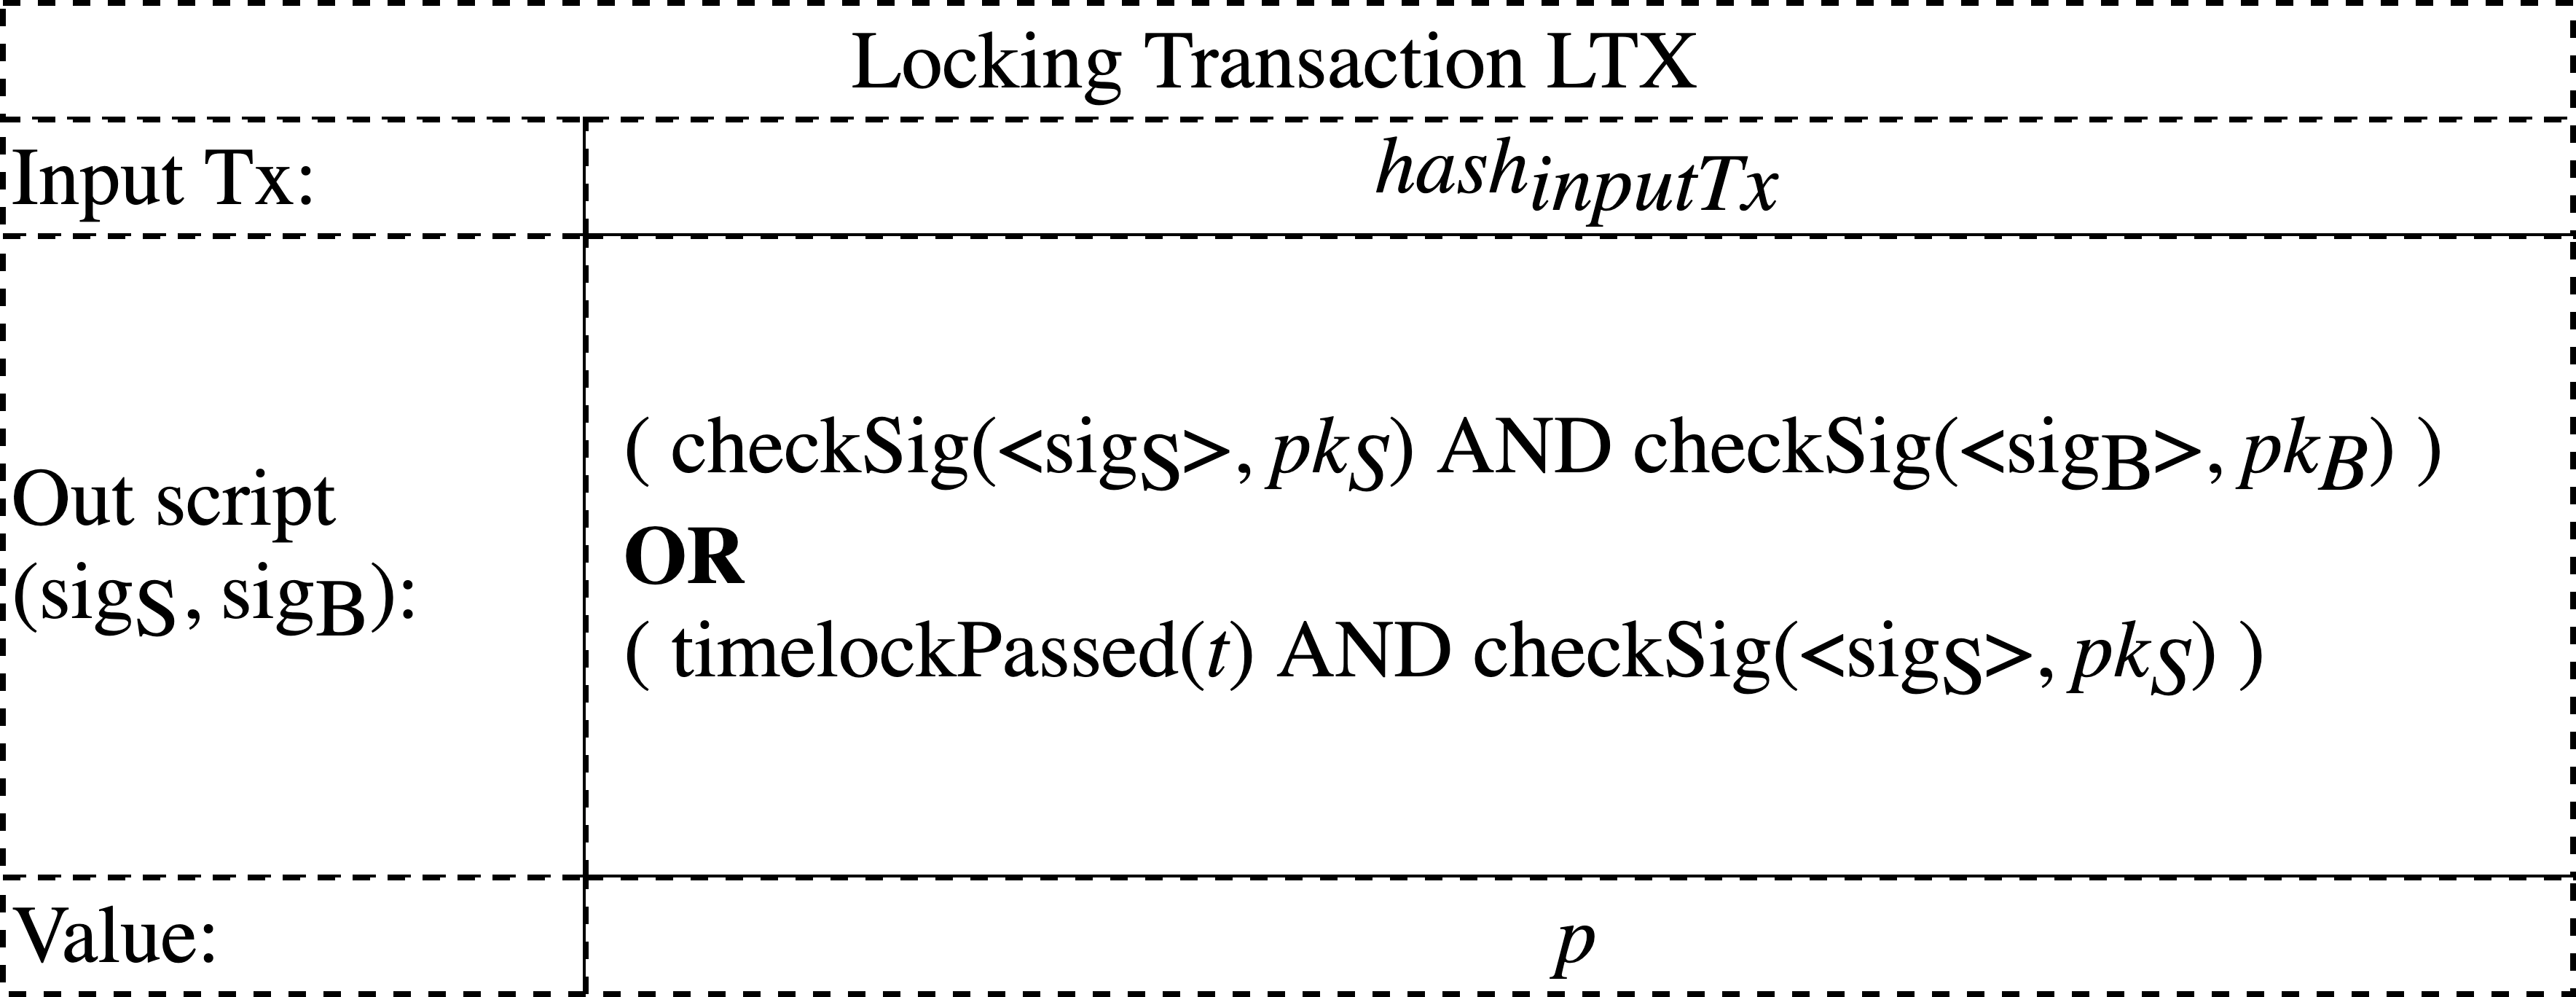
\includegraphics[width=0.61\textwidth]{images/GenLockingTx.png}
              \caption{\textsf{GenLockingTx}$(pk_S, pk_B, t, p)$}
              \label{fig:genLockingTx}
            \end{center}
        \end{figure}
        
        \begin{figure}
            \begin{center}
              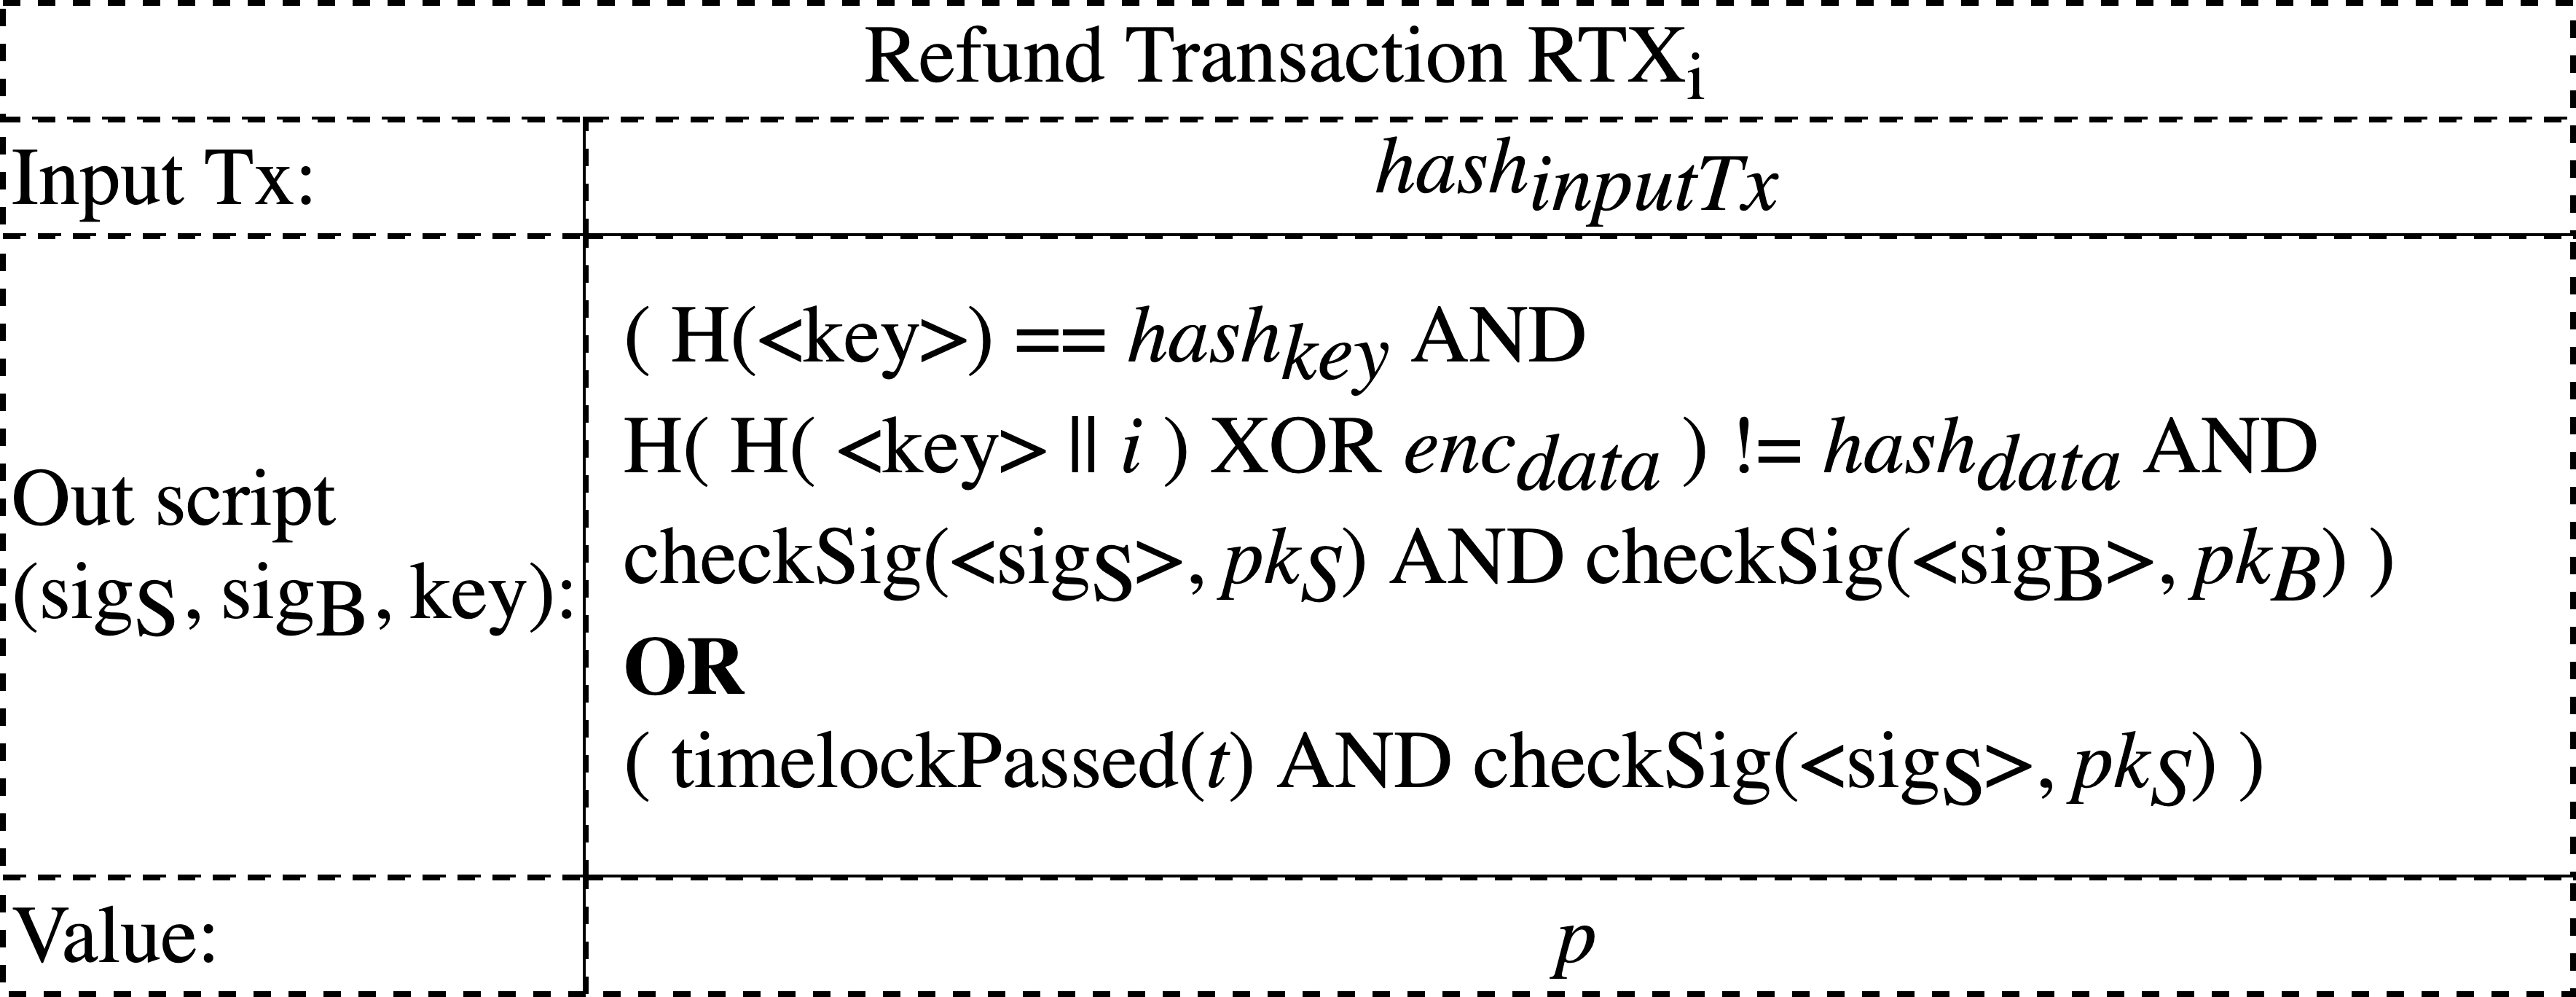
\includegraphics[width=0.61\textwidth]{images/GenRefundTx.png}
              \caption{\textsf{GenRefundTx}$(hash_{inputTx}, pk_S, pk_B, hash_{key}, hash_{data}, enc_{data}, i, t, p)$}
              \label{fig:genRefundTx}
            \end{center}
        \end{figure}
        
        \begin{figure}
            \begin{center}
              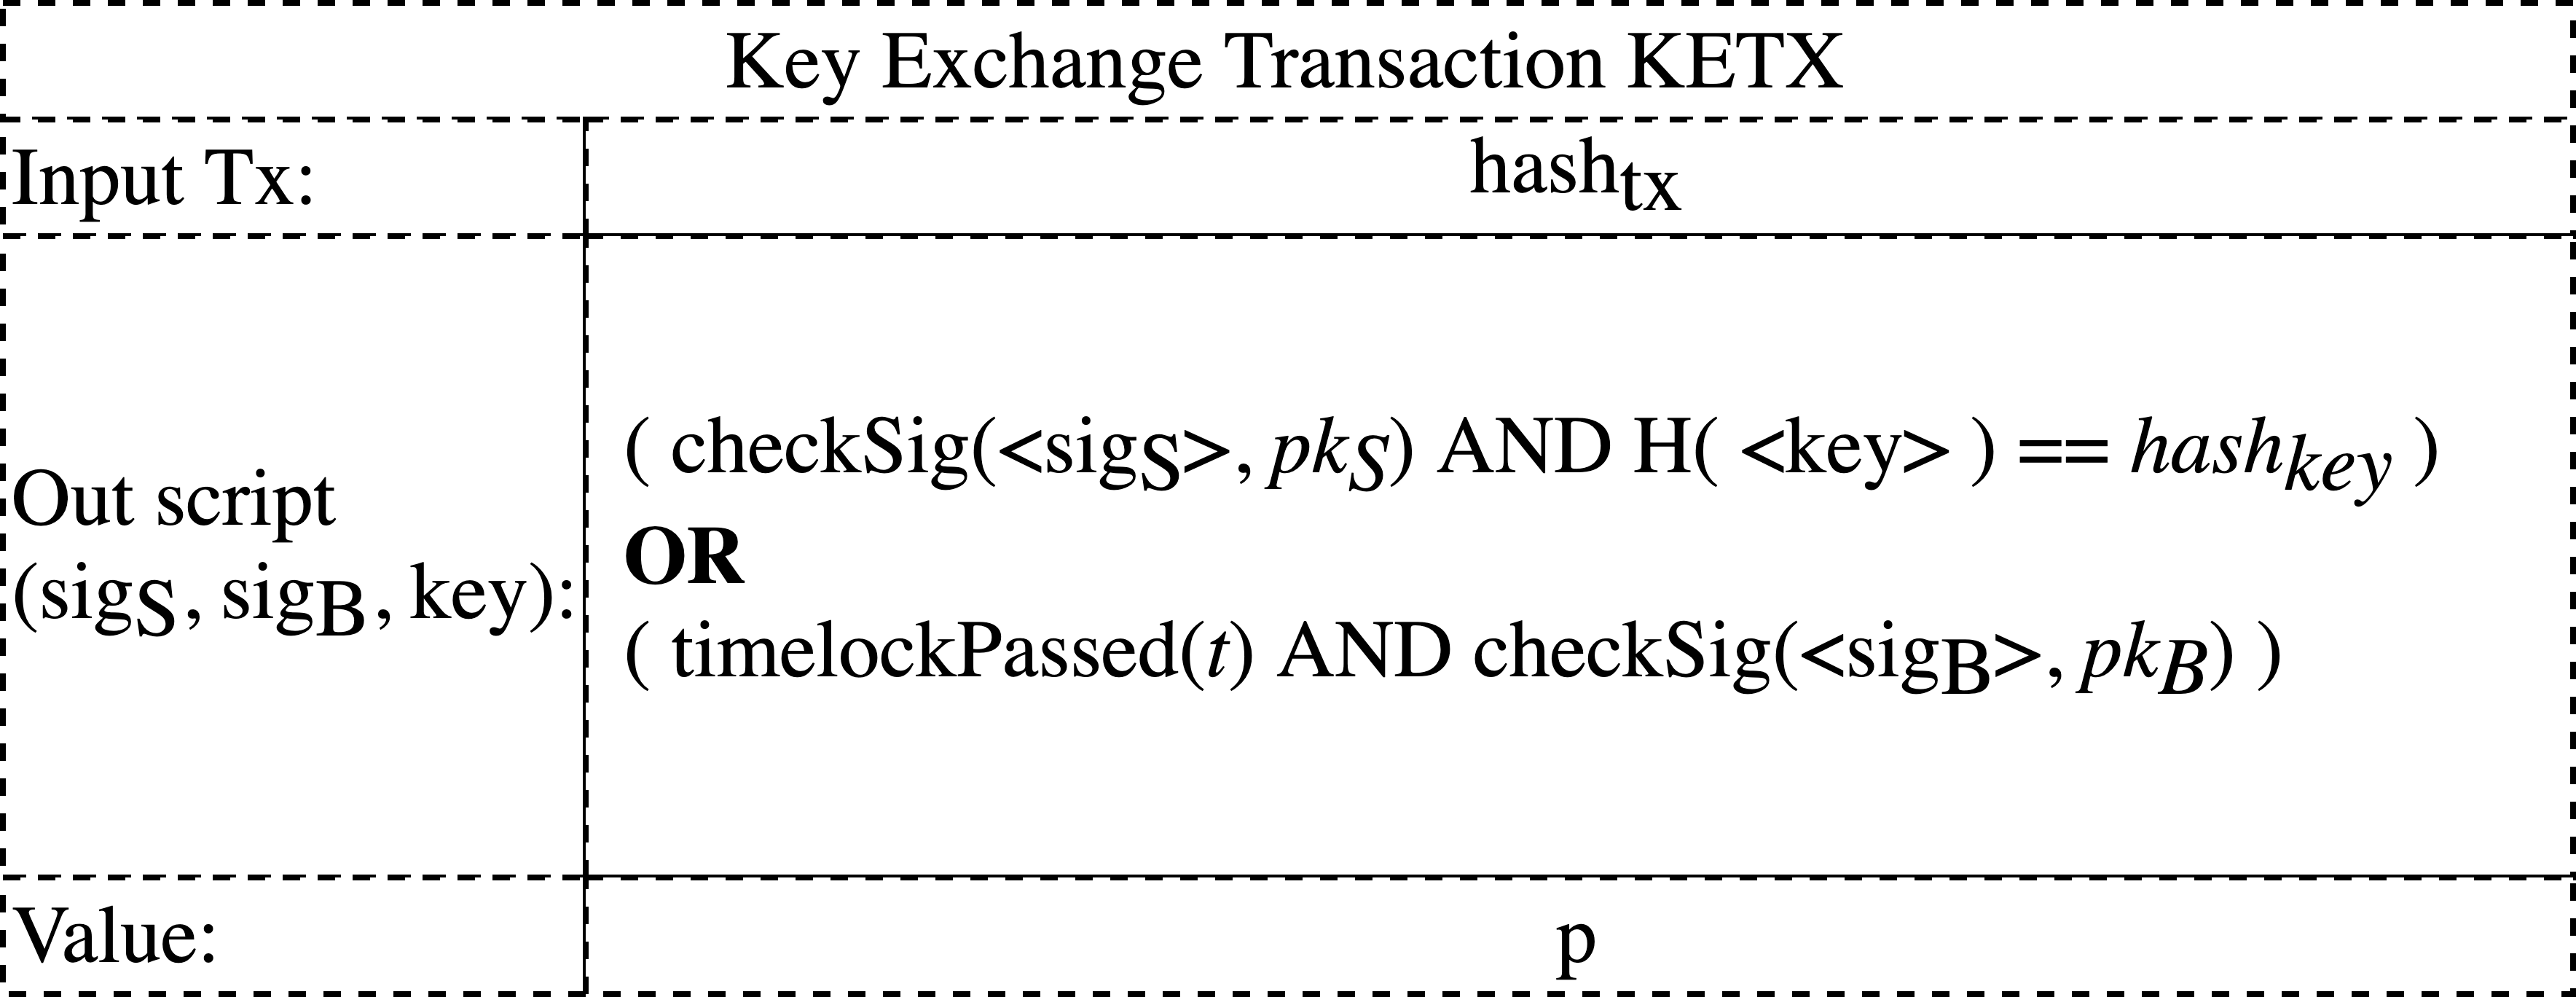
\includegraphics[width=0.61\textwidth]{images/GenKeyExchangeTx.png}
              \caption{\textsf{GenKeyExchangeTx}$(pk_S, pk_B, hash_{key}, t, p)$}
              \label{fig:genKeyExchangeTx}
            \end{center}
        \end{figure}
        
        \section{Algorithms}
        \label{sec:ourAlgos}
        Let us define the following three utility algorithms \textsf{Encoding}, \textsf{Decoding} and \textsf{ConsistencyCheck} utilized by our protocol:
        \subsection{Encoding}
        The \textsf{Encoding} algorithm takes data $\textsf{\textbf{x}} = (\textsf{x}_1, ..., \textsf{x}_c) \in (\{0,1\}^m)^c$ and key $k$. Each chunk of \textsf{\textbf{x}} is encrypted according to the symmetric encryption scheme defined in \ref{sub:SymmetricEncryptionScheme}, with $i$ being the index value. Notably, each encrypted data chunk \textsf{\textbf{ex}}$_i$ got encrypted with and individual key $k_i$ dependent on its index $i$ in \textsf{\textbf{x}}. Additionally to \textsf{\textbf{ex}} this function returns the hash of $k$.
        \begin{center}
        \begin{minipage}[t]{4in}
            \begin{algorithm}[H]
                \ForEach{$i \in (1, ..., |\normalfont{\textsf{\textbf{x}}}|)$}{
                $k_i = H(k \| i)$\;
                $\textsf{ex}_i = k_i \oplus \textsf{x}_i$\;
                }
                $\textsf{\textbf{ex}} = (\textsf{ex}_1,..., \textsf{ex}_{|\textsf{x}|})$\;
                $hash_k = H(k)$\;
                \Return $(\textbf{ex}, hash_k)$\;
                \caption{\textsf{Encode($\textbf{x}, k$)}}
            \end{algorithm}
        \end{minipage}    
        \end{center}
        
        \subsection{Decoding}
        The \textsf{Decoding} algorithm decrypts given $\textsf{\textbf{ex}} = (\textsf{ex}_1, ..., \textsf{ex}_c) \in (\{0,1\}^m)^c$ with $k$ on par with the \textsf{Encoding} algorithm. Therefore it recreates the individual keys $k_i$ from the data chunks to attain \textsf{\textbf{x}}. Additionally, the algorithm generates the Merkle tree of resulting \textsf{\textbf{x}} and compares it to the given Merkle tree  $M_\textsf{x}$. If the roots match, \textsf{\textbf{x}} is considered valid and returned. Otherwise, the first invalid chunk $i$ of \textsf{\textbf{x}} is attained through the verification of Merkle proofs. In this case, besides (invalid) \textsf{\textbf{x}},  the index $i$ is returned.
        \begin{center}
        \begin{minipage}[t]{4in}
            \begin{algorithm}[H]
                 \ForEach{$i \in (1, ..., |$\textsf{\textbf{ex}}$|)$}{
                  $k_i = H(k \| i)$\;
                  $\textsf{x}_i = k_i \oplus \textsf{ex}_i$\;
                 }
                 $\textsf{\textbf{x}} = (\textsf{x}_1,..., \textsf{x}_{|\textsf{\textbf{ex}}|})$\;
                 $M_\textsf{x}' = $ \textsf{Mtree}$(\textsf{\textbf{x}})$\;
                 \If{$root(M_{\normalfont{\textsf{x}}}') \neq root(M_{\normalfont{\textsf{x}}})$}{
                    \ForEach{$i \in (1, ..., |\textsf{\textbf{ex}}|)$}{
                        $p_i = $ \textsf{Mproof}$(M_\textsf{x}, i)$\;
                        \If{\normalfont{\textsf{Mvrfy}}$(\textsf{x}_i, p_i, root(M_\textsf{x})) = 0$}{
                            \Return $(\textsf{\textbf{x}}, i)$\;
                        }
                    }
                }
                \Return $(\textsf{\textbf{x}}, \perp)$\;
                \caption{\textsf{Decode($\textbf{ex}, k, M_\textsf{x}$)}}
            \end{algorithm}
        \end{minipage}
        \end{center}
        
        \subsection{Consistency Check}
        The \textsf{ConsistencyCheck} algorithm takes a reference set of RTX \textbf{TX} and creates another set \textbf{TX'} with the input values. If these sets are identical, the check passed, and the algorithm returns \textsf{true}. Otherwise, the algorithm returns \textsf{false}.
        
        \begin{center}
        \begin{minipage}[t]{4in}
            \begin{algorithm}[H]
                $c = |\textbf{TX}|$\;
                \ForEach{$i \in (1, ..., c)$}{
                $l_i$ = $leaf_i$($M_{\normalfont{\textsf{x}}}$)\;
                $TX_i$ $\leftarrow$ \textsf{GenRefundTx($hash_{tx'}, pk_S, pk_B, hash_k, l_i,\textsf{ex}_i, i, t, p$)}\;
                }
                \textbf{TX'} $ = ( TX_1, ..., TX_c)$\;
                \If{\normalfont{\textbf{TX'} \neq \textbf{TX}}}{
                \Return $\textsf{false}$\;}
                \Return $\textsf{true}$;
                \caption{\\\mbox{\textsf{ConsistencyCheck(}\textbf{TX}\textsf{$, hash_{tx'}, pk_S, pk_B, hash_{k}, M_{\normalfont{\textsf{x}}}, \textbf{\textsf{ex}}, t, p$)}}}
            \end{algorithm}
        \end{minipage}    
        \end{center}
        
        \newpage
        
        \section{Protocol Description}
        We realize the exchange of a product $\textsf{x}$ between seller $S$ and the buyer $B$ for price $p$ in protocol \ref{theProtocol}. In preparation for the exchange, $\textsf{x}$ is split up into $c$ chunks of data (= $\textsf{\textbf{x}}$). We assume that $|\textsf{\textbf{x}}| = m*c $ where $m$ is representing the size of each chunk. At the beginning of the protocol, the Merkle tree of $\textsf{\textbf{x}}$ ($M_x$) is available to both parties as public knowledge. The Merkle tree leaves are the hashed chunks of $\textsf{\textbf{x}}$. Therefore, $B$ does not learn anything about $\textsf{\textbf{x}}$, besides its size. (Note that $M_x$ differs for the same $\textsf{\textbf{x}}$ if a different split $c$ is chosen.) Additionally, three (to the start time of the protocol) relative timelocks $t_{lock}, t_{refund}, t_{claim}$ are known to both parties. We require that $t_{lock} > t_{refund} > t_{claim}$. \\\\
        To encrypt $\textsf{\textbf{x}}$, $S$ creates a new secret key $k$ and performs the \textsf{Encoding} routine, which generates $\textsf{\textbf{ex}}$ (encrypted $\textsf{\textbf{x}}$) and $hash_k$ (the cryptographic hash of $k$). Then, $S$ lockes up $p$ coins via the Locking Transaction $TX_{lock}$ to eventually fund one of $i \in (1, ..., c)$ new Refund Transactions $TX_{{refund}_i}$. ($TX_{lock}$  is used as input transaction for each $TX_{{refund}_i}$. By creating each $TX_{{refund}_i}$ with the correct values, $S$ makes sure that these transactions remain unspendable for $B$.) We will refer to the $c$ Refund Transactions as \textbf{TX$_{{refund}}$}. For the next step $S$ sends \textbf{TX$_{{refund}}$}, including $S$'s signature for the out script's, to $B$. Note that this implicitly shares $\textsf{\textbf{ex}}$ with $B$. Finally $S$ publishes $TX_{lock}$ to the ledger to fully initiate the protocol's refund functionality. This is visualized in Figure \ref{fig:lockingRefundTx}. \\\\
        $B$ receives \textbf{TX$_{{refund}}$} and extracts $\textsf{\textbf{ex}}'$ from the out scripts. We refer to the parsed encrypted data as $\textsf{\textbf{ex}}'$ because $B$ does not know if the encrypted data contains desired $\textsf{\textbf{x}}$ (results in $M_x$). $B$ then validates all Refund Transactions and checks for $TX_{lock}$ on the ledger. If no protocol violation is discovered, $B$ proceeds. The actual data is already exchanged but without $k$ not accessible for $B$. To attain $k$, $B$ creates the Key Exchange Transaction $TX_{exch}$ that locks $p$ coins through $hash_k$ and publishes it to the ledger. \\\\
        $S$ waits for $TX_{exch}$ to appear on the ledger. If this does not happen until $t_{claim}$, $S$ assumes that $B$ aborted the protocol and waits until $t_{lock}$ to claim $TX_{lock}$ and leave the protocol. This could potentially fail if $TX_{lock}$ is already spent by $B$ and implies that one of the Refund Transactions in \textbf{TX$_{{refund}}$} got published to the ledger. If this is the case, $S$ claims $TX_{{refund}_i}$. $S$ is able to do this, because $t_{refund}$ is passed at this point. If $TX_{exch}$ does appear on the ledger, $S$ claims $p$ coins through $TX_{exch}$ by providing $k$ s.t. $H(k) = hash_k$. The exchange is finished for $S$ and $S$ only needs to wait until $t_{lock}$ to claim the locked coins in $TX_{lock}$ back. \\\\
        $B$ waits for the spending of $TX_{exch}$ by $S$ to learn $k$. If this does not happen in time (until $t_{claim}$) $B$ assumes $S$ aborted the protocol, claims $TX_{exch}$ back and aborts. Otherwise, $B$ parses $k$ and decrypts $\textsf{\textbf{ex}}'$ through the \textsf{Decoding} routine and attains $\textsf{x}'$. If the expectation ($M_x$) is met, $\textsf{x}' = \textsf{x}$ and the exchange was successful. If this is not the case, the \textsf{Decoding} routine outputs the index $i$ of the (first) unexpected data chunk in $\textsf{x}'$. This enables $B$ to publish and claim $TX_{{refund}_i}$ by providing $k$ to its out script. We will show this informally in the following Section \ref{sec:Security}. 


        
        
        \begin{figure}
            \begin{center}
                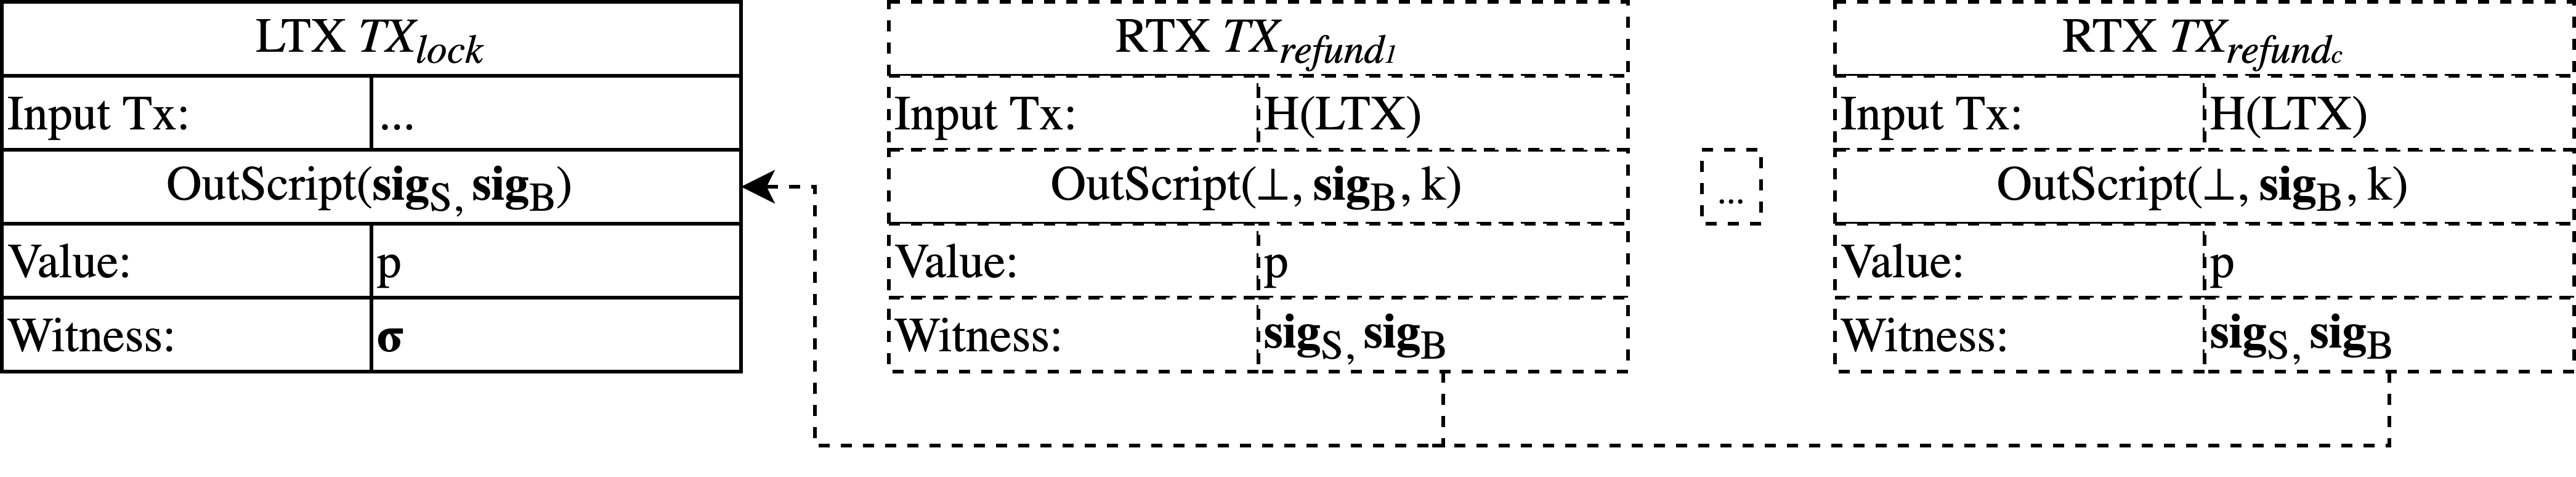
\includegraphics[width=\textwidth]{images/locking_refund_tx_figure.png}
              \caption{Transaction structure of the refund functionality}
              \label{fig:lockingRefundTx}
            \end{center}
            \end{figure}
            
        
        \begin{protocol}{The Fair Exchange Protocol}
        Let $H(\cdot)$ be an collision resistant Hash-Function, $n$ the security parameter and $m$ the data chunk size. \sbline
        \textit{Public information.} $(M_x, p, pk_S, pk_B, t_{lock}, t_{refund}, t_{claim})$
        \sbline
        \textit{Seller \normalfont{S} Input.} $(\textsf{\textbf{x}} = (\textsf{x}_1, ..., \textsf{x}_c) \in (\{0,1\}^m)^c)$
        \sbline
        \textit{Buyer \normalfont{B} Input.} $()$
        \sbline
        \textit{The protocol:}
          \begin{enumerate}
            \item Round (S)
            \begin{enumerate}
    	        \item S generates secret key $k$ $\leftarrow$ $\{0, 1\}^n$ uniformly at random.
            
                \item S computes $(\textsf{\textbf{ex}} = (\textsf{ex}_1, ..., \textsf{ex}_c), hash_k)$ $\leftarrow$ \textsf{Encode}(\textsf{\textbf{x}}$, k$).
            
                \item S creates Locking Transaction $TX_{lock}$ $\leftarrow$ \textsf{GenLockingTx($pk_S, pk_B, t_{lock}, p$)}.
            
                \item For each $i \in (1, ..., c)$, S creates a new Refund Transaction \mbox{$TX_{{refund}_i}$ $\leftarrow$ \textsf{GenRefundTx($H(TX_{lock}), pk_S, pk_B, hash_k, H(\textsf{x}_i), \textsf{ex}_i, i, t_{refund}, p$)}}.
                
                \item S sends the signed set \textbf{TX$_{{refund}}$} $ = ( TX_{{refund}_1}, ..., TX_{{refund}_c})$ to B and publishes $TX_{lock}$ with \textsf{PublishToLedger($TX_{lock}$)}.
            \end{enumerate}
            
            \item Round (B)
            \begin{enumerate}
                \item B parses $\textsf{\textbf{ex}}'$ from \textbf{TX$_{{refund}}$}.
                \item B evaluates \textsf{ConsistencyCheck(}\textbf{TX$_{{refund}}$}\textsf{$, H(TX_{lock}), pk_S, pk_B, hash_k, M_x, \textsf{\textbf{ex}}', t_{refund}, p$)} and \textsf{IsOnLedger($TX_{lock}$)}. If one or more checks fail, B aborts and the exchange failed.
                \item If $t_{refund}$ passed, B aborts and the exchange failed.
            \end{enumerate}
            
          \newcounter{enumTemp}
          \setcounter{enumTemp}{\theenumi}
          \end{enumerate}

          \begin{enumerate}
          
          \begin{enumerate}
             \setcounter{enumii}{3}
            \item B creates Key Exchange Transaction $TX_{exch}$ $\leftarrow$ \textsf{GenKeyExchangeTx($pk_S, pk_B, hash_k, t_{claim}, p$)}. $TX_{exch}$ is then published with \mbox{\textsf{PublishToLedger($TX_{exch}$)}}.
          \end{enumerate}
            
            \setcounter{enumi}{\theenumTemp}
            
            \item Round (S)
            
            \begin{enumerate}
            \item If $t_{claim}$ passed, S waits for $t_{lock}$ and claims $TX_{lock}$ via \textsf{Claim($TX_{lock}, \perp$)}. If this fails and $TX_{lock}$ is already spent through one $TX_{{refund}_i} \in$ \textbf{TX$_{{refund}}$}, S claims this transaction via \textsf{Claim($TX_{{refund}_i}, \perp$)}. S, therefore, aborts and the exchange failed. 
            
            \item S claims $TX_{exch}$ by running \textsf{Claim($TX_{exch}, k$)} and earns p coins.
            \end{enumerate}
            
            \item Round (B)
            \begin{enumerate}
            \item If $t_{claim}$ passed and $TX_{exch}$ unspent, B reclaims $TX_{exch}$ via \textsf{Claim($TX_{exch}, \perp$)}, therefore, aborts and the exchange failed. 
            
            \item B parses $k$ from $TX_{exch}$ and computes $(\textsf{\textbf{x}}', i)$ $\leftarrow$ \textsf{Decode(}$\textsf{\textbf{ex}}'$\textsf{$, k, M_x$)}. 
            \end{enumerate}
            
          \newcounter{enumTemp}
          \setcounter{enumTemp}{\theenumi}
          \end{enumerate}
          
          \begin{enumerate}
          \setcounter{enumi}{\theenumTemp}
            \begin{enumerate}
            \setcounter{enumii}{2}
            \item If $i \neq \perp$ B publishes $TX_{{refund}_i}$ via \textsf{PublishToLedger($TX_{{refund}_i}$)} to implicitly claim $TX_{lock}$. B runs \textsf{Claim($TX_{{refund}_i}, k$)} to ultimately secure the refund, therefore, aborts and the exchange failed. 
            
            \item B concatenates all elements of $\textsf{\textbf{x}}'$ to attain $\textsf{x}' = \textsf{x}$ and the exchange was successful.
            \end{enumerate}
            
          \end{enumerate}
          \label{theProtocol}
        \end{protocol}
        
        \section{Security}
        \label{sec:Security}
        In this section, we conduct an informal security analysis of the given protocol. We say that the protocol is secure if the \textit{seller security} property and \textit{buyer security} property hold. We assume the protocol is sender secure if it is guaranteed that the buyer $B$ only learns the product \textsf{x}, if and only if $B$ pays $p$ coins to seller $S$. We assume that the protocol is buyer secure if an honest $B$ is ensured that if he pays $p$ coins to $S$, $B$ will receive the expected product \textsf{x} or at least a compensation (refund) of $p$ coins. We will ignore transaction fees in the following. \\\\
        Notice that our protocol consists of two main functionalities: On the one hand, there is the Key Exchange Transaction, and on the other hand, the \textit{refund functionality} consisting of the set of Refund Transactions funded by the Locking Transaction. The Key Exchange Transaction guarantees the \textit{seller security} property trivially if we assume the \textsf{Encoding} and \textsf{Decoding} algorithms' correctness (s.t. \textsf{Decode(Encode(}\textsf{x$, k$)}$, k, M_x$\textsf{)} = $($\textsf{x}$, \perp)$) and the security of the symmetric encryption scheme (cf. §\ref{sub:SymmetricEncryptionScheme}). The transaction enables $S$ to share the secret key $k$ (that allows $B$ to lean the product) atomically in exchange for $p$ coins. \\\\
        Next, we will look into the \textit{buyer security}. Assume $S$ is honest, then this property holds for the same reason the \textit{seller security} has, and $B$ will receive the secret key $k$ and thereby is able to learn the expected product. Otherwise, if $S$ is malicious, the \textit{buyer security} holds because one of the Refund Transactions is guaranteed to become spendable for $B$ once the key exchange happened and $p$ coins were transferred to $S$. We will show that this is the case with the following examples. Note that each Refund Transaction out script resembles the decryption and hashing of a particular encrypted data chunk. The solved out script would prove $S$' misbehavior. It is only solvable if the correct secret key is provided by $B$ and the computed hash does not equal the specific Merkle tree leave of \textsf{x}.
        \begin{enumerate}
            \item Let us assume $S$ tries to send a wrong secret key $k^*$. Its hash must be consistent across the Refund Transaction set because otherwise $B$ would notice this in step 2b) and abort. If the hash is consistent, $B$ creates the Key Exchange Transaction based on it in 2d) and will receive $k^*$ if $S$ wants to claims the $p$ coins. Therefore, every Refund Transaction is spendable for $B$ because the hash of $k^*$ matches, but the hash of the decoded data chunk inside the out script does not equal its expected Merkle tree leaf.

            \item Let us assume $S$ sends the correct key $k$ but manipulated the i-th data chunk of encrypted \textsf{\textbf{ex}}, s.t. $B$ does not receive the expected \textsf{x} after decoding. In this case, $B$ won't notice anything in the respective $i$-th Refund Transaction because the included Merkle tree leaf is still correct. Therefore the Key Exchange Transaction is published, spent by $S$ and  $B$ receives $k$.  The \textsf{Decoding} algorithm will output the manipulated data chunks index $i$ in step 4b). Thereby, the $i$-th Refund Transaction must be spendable because the hash of $k$ matches, but the hash of the decoded data chunk inside the out script does not equal the expected $i$-th Merkle tree leaf.

            \item Another option for a malicious $S$ to cheat would be by manipulating the expected Merkle tree leaves inside the Refund Transactions to make one of the two attacks above possible. Because the Merkle tree of \textsf{x} is public knowledge, this is not possible and is noticed by $B$ in step 2b). 
        \end{enumerate}
        Because of the design of the Refund Transactions we consider the \textit{buyer security} property to be met. \\\\
        Finally, we want to stress that correct timestamps (s.t. $t_{lock} > t_{refund} > t_{claim}$) are essential for the security of the protocol. Only under this condition, the \textit{refund functionality} works properly. Otherwise, the Refund Transactions could become unpublishable because there is no unspent input transaction. Also note, that after publishing one Refund Transaction, all others become unpublishable because the Locking Transaction is spent. Although $S$ might behave honestly, a malicious $B$ is eventually able to publish one of the Refund Transaction without the ability to spend it by himself. This case can be considered a \textbf{griefing attack}, as discussed briefly in Section \ref{sub:Results}. Therefore the Locking Transaction and each Refund Transaction must be claimable for $S$ after the respective timelock passed. This is part of the following fairness discussion.


        
        \section{Fairness Discussion}
        \label{sec:FairnessDiscussion}
	    Our protocol achieves a decent notion of fairness without one party having a significant advantage over the other. Let us be specific on this in the following, by briefly analyzing a possible advantage according to the general \textit{fairness}, \textit{timeliness}, and \textit{abuse-freeness} introduced in Section \ref{sec:Advantage}: \\\\
        \textbf{General fairness} is fulfilled because the exchange ends with the Key Exchange Transaction, which pays the seller and enables the buyer to learn the product. If the product is the expected on, all parties received their expected result. If the exchanged product is not the expected one, the refund functionality enables the buyer to use the sellers locked coins to compensate for the Key Exchange Transaction payment. Therefore, both parties do not receive anything: $S$ did not make any profit, and the received product is worthless for the buyer. We can derive from this that \textbf{our protocol achieves strong fairness} (cf. §\ref{sec:StrongFairnessWeakFairness}). \\\\
        We regard the \textbf{timeliness} property to be essentially fulfilled through the utilized time locks. These enable to pre-define a specific time window in that certain actions are expected from the opposite party. Therefore, the progress of the protocol and the abortion of a party is easily observable. Note that once coins are locked (e.g., through the Locking Transaction or the Key Exchange Transaction), the party is forced to stay inside the protocol until the respective timelock passed to recover the coins. Although, in that case, a party cannot directly abort the protocol, we do not regard this as a violation of the timeliness property because the locked coins do not need to be actively preserved. Therefore they can be regarded as an unspent \textit{P2PKH} transaction. \\\\
        Our protocol does not provide \textbf{abuse-freeness}. From the buyers point of view, abuse-freeness holds because the seller needs to lock coins beforehand to proceed in the exchange. Therefore, the seller is required to pay fees and is incentivized to continue. Because of the same scenario, abuse-freeness does not hold for the seller because there is no incentive (despite receiving the product) that stops the buyer from aborting right after the Locking Transaction is published. Another opportunity for abuse by the buyer is to publish one Refund Transaction, despite not being able to spend it. This increases the total transaction costs for the seller. Despite this, note that until the Key Exchange transaction is published, no single party has the power to complete the protocol successfully without the cooperation of the other party. \\\\
        Let us briefly analyze the advantages of transaction fees one party might have over the other: In the optimistic case, both parties are required to publish one transaction each. Therefore, the transaction fees are equally split. If the refund functionality is utilized, the buyers additional transaction is published, and additional fees are being paid. An easy solution to this imbalance (especially because the seller is considered malicious in this scenario) is that the locking transaction's value could be set higher than the product's actual price. \\\\
        Finally, we do not see any mentionable advantage for a single party in terms of computational effort. Despite no heavy cryptographic task required to run our protocol, the computational effort is relatively balanced. 
	    
	\chapter{Implementation}
	    In order to validate the proposed protocol and learn about its real-world costs, we implement a test bench\footnote{\url{https://github.com/leandro-ro/bt-evaluation}} that includes the presented transaction types and algorithms. We define and run five different scenarios on-top of this test bench. Due to the fact that our protocol only utilizes simple cryptographic operations (that are expected to run fast and efficiently on modern hardware) we focus our evaluation on the transaction fees rather the computational complexity. Please note that the protocol is currently not feasible on Bitcoins blockchain because we require OP\_XOR and OP\_CAT to decrypt a data chunk inside a Refund Transaction. As we already showed in Table \ref{tbl:opcodes}, these two opcodes are currently disabled in Bitcoin, although there is the chance that the opcodes are being reintroduced through a future BIP. To still be able to evaluate our protocol, we utilize Bitcoin Cash (cf. §\ref{sec:BitcoinCash}) instead, which allows the use of mentioned opcodes. What we learn here is directly transferable to Bitcoin itself because both blockchains run on the same Bitcoin Script language (cf. §\ref{sub:BTCScript}). Hence we do not need to change the implemented transactions if we want to run them on a future Bitcoin version that supports the required opcodes. In both cases, the transaction costs are measured in satoshi\footnote{Smallest unit of Bitcoin (Cash): 1 sat = 0,00000001 BTC/BCH} per byte; therefore, the single important metric we want to evaluate is the size of each transaction type.
	    
	    \section{Tools}
        We use JavaScript and a hand full of libraries to conduct the evaluation. Most notably, we utilize the bitcore-lib-cash\footnote{\url{https://github.com/bitpay/bitcore/tree/master/packages/bitcore-lib-cash}} library and the bitbox-sdk\footnote{\url{https://github.com/Bitcoin-com/bitbox-sdk}} for wallet instantiation and interaction with the blockchain. We use Bitcoin Cash's testnet to run all our scenarios on. This enables us to track our submitted transactions via a blockchain explorer\footnote{e.g., \url{https://www.blockchain.com/explorer?view=bch}}. We choose CashScript\footnote{\url{https://cashscript.org/}} to implement the transaction types on a high level for easier fault detection and better understanding. In this context we use meep\footnote{\url{https://github.com/gcash/meep}} for step-by-step transaction debugging. Additionally we utilize merkletreejs\footnote{\url{https://github.com/miguelmota/merkletreejs}} for the implementation of our \textsf{Decoding} algorithm and crypto-js\footnote{\url{https://github.com/brix/crypto-js}} that provides the SHA-256 hash function. \\\\  
        CashScript is already mentioned in Section \ref{sec:smartContractOptions} but let us show how we realized our transaction types through exemplary creating a \textit{P2PKH} transaction (we also utilize this transaction in our implementation): First we create a standard \textit{P2PKH} transaction in CashScript syntax (Listing \ref{lst:p2pkhCashScript}). We use this transaction inside our implementation by first compiling the CashScript file and then creating the transaction via its constructor (Listing \ref{lst:cashScriptInUse}). Based on the arguments passed to the constructor, the CashScript library generates a transaction with the usual Bitcoin Script, which is equivalent to earlier Listing \ref{fig:p2pkh}. After instantiating, we can interact with the transaction and spend it.
	    
	    \begin{minipage}{\linewidth}
	    \definecolor{backcolour}{rgb}{0.95,0.95,0.92}
        \begin{lstlisting}[language=JavaScript, basicstyle=\footnotesize, caption= p2pkh.cash - Bitcoin \textit{P2PKH} in high-level CashScript, captionpos=b, backgroundcolor=\color{backcolour}, label=lst:p2pkhCashScript]
        pragma cashscript ^0.5.0;
        
        contract P2PKH(bytes20 pkh) {
        // Require pk to match stored pkh and signature to match
            function spend(pubkey pk, sig s) {
                require(hash160(pk) == pkh);
                require(checkSig(s, pk));
            }
        }
        \end{lstlisting}
        \end{minipage}
        
        \begin{minipage}{\linewidth}
        \definecolor{backcolour}{rgb}{0.95,0.95,0.92}
        \begin{lstlisting}[language=JavaScript, basicstyle=\footnotesize, caption= Compiling and executing CashScript \textit{P2PKH} via JavaScript , captionpos=b, backgroundcolor=\color{backcolour}, label=lst:cashScriptInUse]
        // Compile a contract file
        const P2PKH = CashCompiler.compileFile(path.join(__dirname, 'p2pkh.cash'));

        const provider = new ElectrumNetworkProvider('testnet');
        const contract = new Contract(P2PKH, [alicePkh], provider);
        
        const tx = await contract.functions
        .spend(alicePk, new SignatureTemplate(alice))
        .to('bitcoincash:qrhea03074073ff3zv9whh0nggxc7k03ssh8jv9mkx', 10000)
        .send()
        \end{lstlisting} 
	    \end{minipage}
	    
	    
	    \section{Scenarios}
	    \label{sec:Scenarios}
	    For this evaluation, we differentiate between five different scenarios. All these scenarios will always need to follow a specific transaction flow (chain of transactions). All paths are presented in Figure \ref{fig:transactionFlow}. Note that due to the transactions out scripts and the requirement that an input transaction needs to be unspent (cf. §\ref{sub:BTCTx}), not all combinations are possible. For example, transaction c cannot exist alongside transaction f on the blockchain (if we assume the transactions only provide one output).
	    \\\\
	    We define the scenarios as follows:
	    \begin{enumerate}
            \item Scenario - The optimistic case: The buyer publishes the Key Exchange Transaction (b). The seller provides the key to unlock the Key Exchange Transaction (e) and reclaims the locked coins inside the Locking Transaction (a, f).

            \item Scenario - Seller aborts: The seller does not provide the key. Therefore the buyer reclaims his Key Exchange Transaction (b, d). The seller reclaims the locked coins inside the Locking Transaction (a, f).

            \item Scenario - Seller is malicious: The seller publishes the Locking Transaction (a). The buyer publishes the Key Exchange Transaction (b). The seller uses the key to unlock the Key Exchange Transaction (e) but provides manipulated data. Therefore, the buyer publishes the respective Refund Transaction and claims it (c, h).
            
            \item Scenario - Buyer aborts: The seller publishes the Locking Transaction (a). The buyer does not publish the Key Exchange Transaction. The seller reclaims the locked coins inside the Locking Transaction (f).
            
            \item Scenario - Buyer is malicious: The seller publishes the Locking Transaction (a). Without publishing a Key Exchange Transaction, the buyer publishes one (for the buyer undependable) Refund Transaction. The seller reclaims the locked coins inside the Refund Transaction (c, g). Remember, this scenario is indeed a possible one, as described in Section \ref{sec:FairnessDiscussion}.
        \end{enumerate}
	    For a visual representation of each scenario, we refer to our evaluations GitHub repository\footnote{\url{https://github.com/leandro-ro/bt-evaluation}}.
	    
	    
	    \section{Evaluation}
	    \label{sub:eval}
	    As we already mentioned, the costs for a transaction directly result from its size. The transaction size is calculated from two parts. The first one is the transaction without the witness, which is always constant relative to the input transaction. The second one is the witness itself which size might vary based on our protocol parameters. Our protocol's main parameters are the size of the key (= $|key|$) and the size of the data chunks (= $chunkSize$). Although the data chunk size is irrelevant for the optimistic case, we intend to choose relatively small data chunks (up to 32 Bytes) in order to keep the transaction costs low for the case that a Refund Transaction is published. Choosing a smaller chunk size directly implies a larger number of chunks. In this context, we stress that the amount of data chunks is not interesting for our evaluation because it does not affect the transactions' size in any way. 
	    
	    \subsection{Transaction Size}
	    In Table \ref{tab:txSizes} we determine the size of each transaction in Bytes. In the next step to evaluate the full transaction costs, we add the sizes together based on the specific scenario. Our results are displayed in Table \ref{tab:scenarioSizes}. Note that the allocation of a specific transaction to the seller or buyer does not necessarily mean that this party published the transaction. It rather indicates that the party must pay the transaction fees. This might also be the case if another party is responsible for the published transaction, e.g., transaction c in Scenario 5., which is published by the malicious buyer and forces the seller to publish transaction g and therefore pay a transaction fee. The key result of the size determination is that considering a reasonable data chunk size (e.g., 32 Bytes) and key length (e.g., 256 bit = 16 Bytes), the protocol's parameters barely affect the total transactions size and therefore fees, as we present in the next subsection.
	    
	    \begin{table}[]
        \centering
        \begin{tabular}{l|l|l}
        ID & Transaction Type & Size (in Byte)     \\ \hline
        a  & Locking          & $241$                  \\
        b  & Key Exchange     & $241$                  \\
        c  & Refund           & $365$                  \\
        d  & P2PKH            & $304$                  \\
        e  & P2PKH            & $304 + |key|$          \\
        f  & P2PKH            & $265$                  \\
        g  & P2PKH            & $365 + chunkSize$  \\
        h  & P2PKH            & $365 + |key| + chunkSize$
        \end{tabular}
        \caption{Transaction sizes relative to the key length (= $|key|$) and the chunk size (= $chunkSize$)}
        \label{tab:txSizes}
        \end{table}
        
        \begin{table}[]
        \centering
        \begin{tabular}{l|l|l|l|l}
        Scenario               & Tx Seller & Tx Buyer & Seller Tx Size (in Byte) & Buyer Tx Size (in Byte)     \\ \hline
        1. The optimistic case & a, f, e   & b        & $810 + |key|$            & $241$                       \\
        2. Seller aborts       & a, f      & b, d     & $506$                    & $545$                       \\
        3. Seller is malicious & a, e      & b, c, h  & $545 + |key| $           & $971 + |key| + chunkSize$ \\
        4. Buyer aborts        & a, f      & -        & $506$                    & $0$                         \\
        5. Buyer is malicious  & a, c, g   & -        & $971 + chunkSize$      & $0$                        
        \end{tabular}
        \caption{Accumulated transaction sizes based on the five scenarios}
        \label{tab:scenarioSizes}
        \end{table}

        \begin{table}[]
        \centering
        \begin{tabular}{l|l|l|l|l|l|l}
                 & \multicolumn{2}{c|}{Bitcoin Fee} & \multicolumn{2}{c|}{Bitcoin Cash Fee} & \multicolumn{2}{c}{Parameter Impact} \\ \hline
        Scenario & Seller Fee      & Buyer Fee      & Seller Fee        & Buyer Fee         & $|key|$            & $chunkSize$            \\ \hline
        1        & \$16,56         & \$4,82         & \$0,004140        & \$0,001205        & 1,5\%              & 0\%                    \\ 
        2        & \$10,12         & \$10,90        & \$0,002530        & \$0,002725        & 0\%                & 0\%                    \\ 
        3        & \$11,22         & \$2,18         & \$0,002805        & \$0,000545        & 2.0\%              & 2,0\%                  \\ 
        4        & \$10,12         & \$0,00         & \$0,002530        & \$0,000000        & 0\%                & 0\%                    \\ 
        5        & \$20,06         & \$0,00         & \$0,005015        & \$0,000000        & 3,2\%              & 0\%                   
        \end{tabular}
        \caption{\centering Fees for $|key|$ = 256 Bit and $chunkSize$ = 32 Bytes assuming\\1 BTC = \$50.000,00 and 1 BCH = \$500,00}
        \label{tab:feeExample}
        \end{table}
	    
	    \subsection{Protocol Fees}
        Based on our findings in Table \ref{tab:scenarioSizes} we can derive the actual scenario costs. On the day of writing, the average Bitcoin transaction costs are around 40 sat/Byte, and the average Bitcoin Cash transaction costs at 1 sat/Byte. Therefore a party needs to pay 0.00000040 BTC per Byte on Bitcoin or 0.00000001 BCH per Byte on Bitcoin Cash for submitting a transaction. We assume a Bitcoin price of 50000\$ and a Bitcoin Cash price of 500\$ and choose a reasonable chunk size of 32 Bytes and a key length of 256 Bits (= 16 Bytes). The costs for all scenarios under these conditions are presented in Table \ref{tab:feeExample}. As expected, the impact of the key length and chunk size is minimal in relation to the total cost. The spread between Bitcoin and Bitcoin Cash is exceptionally high, with Bitcoin being 4000 times more expensive. This directly results from the 40 times higher sat/Bytes fee and 100 times higher market price of Bitcoin ($40 * 100 = 4000$).
	    
	    \subsection{Results}
	    \label{sub:Results}
	    We learn a few interesting attributes of the protocol through this evaluation.
	    
        \begin{enumerate}
        
        \item On the one hand, we can observe that the protocol transaction costs on Bitcoin itself are very high, making the protocol uninteresting for the exchange of low-cost items. On the other hand, we notice that Bitcoin Cash's transaction costs can almost be considered negligible in our case. Using Bitcoin Cash, our exchange protocol is suitable for low-cost items.
        
        \item The number of data chunks is not affecting the transaction costs. We can conclude that the item's size is only limited by the party's computational power and local storage, not by the blockchain (and the resulting transaction fees) in any way, which is desirable.
        
        \item If we assume an appropriate data chunk size and key length, the transaction fees are barely affected. 
        
        \item The optimistic case's fees are is independent of the data chunk size. This makes the protocol desirable to use with honest or semi-honest parties because the transaction fees will remain constant for any data size (assuming the key length remains the same). Scenario 2. and 3. are unlikely to happen since the aborting/malicious party always looses money.
                    
         \item There are two scenarios (Scenarios 4. and 5.) in which the buyer does not have to pay anything. This fact is the weak spot of the protocol because it enables a malicious buyer to exploit the protocol and harm the seller without fearing any financial consequences (griefing attack). We want to stress that there are possibilities to counteract this behavior in potential future work, e.g., by forcing the buyer into depositing money into the Locking Transaction at the beginning of a protocol run.
         
        \end{enumerate}
	    
	    
	    
	    
	    \begin{figure}
            \begin{center}
                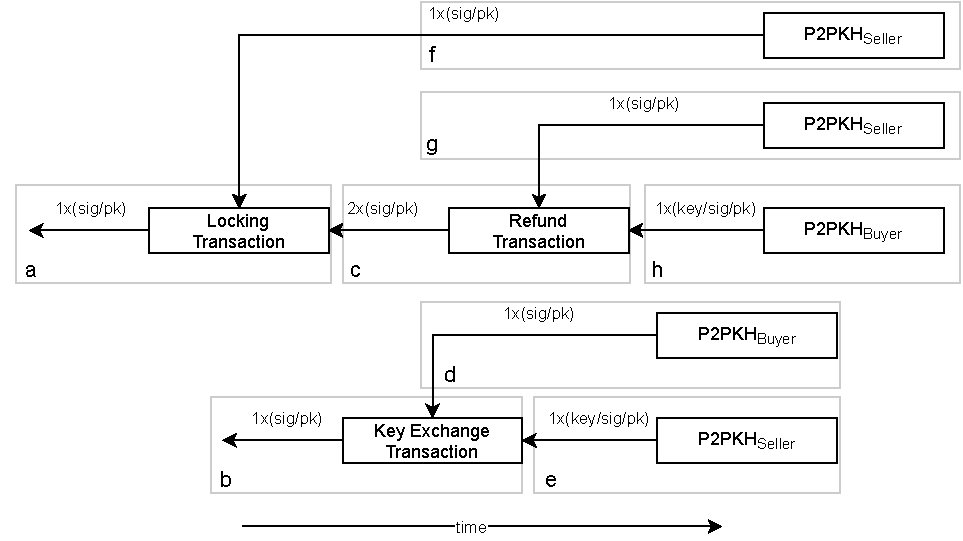
\includegraphics[width=\textwidth]{images/transaction_flow.pdf}
              \caption{Transaction flow of the proposed protocol}
              \label{fig:transactionFlow}
            \end{center}
        \end{figure}
	    
	\chapter{Conclusion}
	\label{sec:Conclusion}
	
	\section{Summary}
    In this thesis, we proposed a protocol for the fair exchange of a digital good between two parties on top of Bitcoin/Bitcoin Cash. We began by analyzing the background and essential aspects of fair exchange protocols in general and took a look at specific protocols (cf. §\ref{sec:relatedWork}). We discovered that it is highly desirable to do as much computation as possible locally instead of on the blockchain, although this does not imply that local computation is negligible. Further, we compared Bitcoin, Bitcoin Cash, and Ethereum respective their abilities when it comes to smart contracts (cf. §\ref{sec:smartContractOptions}). In preparation for our proposed protocol, we described the foundations of Bitcoin and its transactions (cf. §\ref{sec:BTC}). We looked into Ethereum based FairSwap that inspired our proposed protocol with the guiding principle of empowering the buyer to prove the seller's misbehavior after the exchange (cf. §\ref{sec:FairSwap}). After introducing our necessary cryptographic primitives (cf. §\ref{sec:CryptoPrimitives}), we analyzed the current perception of fairness in exchange protocols (cf. §\ref{sec:Fairness}). Besides mentioning types of fairness like Strong and Weak Fairness (cf. §\ref{sec:StrongFairnessWeakFairness}), we learn that fairness is not always sufficiently defined, especially when it comes to the term \textit{advantage} (cf. §\ref{sec:Advantage}). Our protocol construction introduced three new transaction types (cf. §\ref{sec:OurTransactionTypes}): The Locking, Refund, and Key Exchange Transaction. We further defined the \textsf{Encoding}, \textsf{Decoding}, and \textsf{ConsistencyCheck} algorithms (cf. §\ref{sec:ourAlgos}). During the protocol execution, any possibly manipulated data chunk is efficiently discoverable for the buyer. Each data chunk's index directly relates to a specific Refund Transaction that empowers the buyer to claim a refund if he did not receive the expected product. This functionality is achieved with only two custom transaction types in the optimistic case and one additional for the pessimistic case (not counting the standard \textit{P2PKH} transactions). The protocol is secure regarding the buyer and seller security, as informally shown in Section \ref{sec:Security}. Generally, the protocol achieves strong fairness (cf. §\ref{sec:FairnessDiscussion}), but we discovered the risk of griefing attacks by the buyer targeting the seller.  Although this weakness, we recognized desirable properties of the protocol during the evaluation of the implementation's five scenarios (cf. §\ref{sec:Scenarios}): On the one hand, the protocol transaction fees are virtually independent of the item's size, and only simple, computationally cheap cryptographic operations are being utilized. On the other hand, the protocol is realizable on Bitcoin Cash today, with the transaction fees being minimal, making the protocol suitable for microtransactions. The realization on top of Bitcoin itself is questionable. Even if the required opcodes would be reactivated in future BIPs, the transaction costs of custom transaction types are incredibly high.  

    \section{Future Work}
    As mentioned, griefing attack enables the buyer to harm the seller through the transaction costs without paying anything himself. We consider this the weak point of the protocol but see the potential of future work here. Technically, it is possible to change the Locking Transaction so that both parties need to lock money at the beginning of the exchange and, therefore, implicitly commit to it. By providing similar functionality, the risk of griefing attacks would be eliminated because, in every case, the parties are financially involved. Additionally, we identify the protocols space complexity as interesting to be analyzed in future work. Many Refund Transactions need to be created for high numbers of data chunks, with each of them requiring a unique signature from the seller. This has a potentially high impact on the protocols real-world performance in specific cases.
 
    
	
	\newpage
    \bibliographystyle{unsrt}
    \bibliography{ref}
	
	\appendix
\end{document}